%%
%% abtex2-modelo-trabalho-academico.tex, v-1.9.2 laurocesar
%% Copyright 2012-2017 by abnTeX2 group at http://abntex2.googlecode.com/ 
%%
%% This work may be distributed and/or modified under the
%% conditions of the LaTeX Project Public License, either version 1.3
%% of this license or (at your option) any later version.
%% The latest version of this license is in
%%   http://www.latex-project.org/lppl.txt
%% and version 1.3 or later is part of all distributions of LaTeX
%% version 2005/12/01 or later.
%%
%% This work has the LPPL maintenance status `maintained'.
%% 
%% The Current Maintainer of this work is Emílio Eiji Kavamura,
%% eek.edu@outlook.com; emilio.kavamura@ufpr.br
%% Further information about abnTeX2 are available on 
%%
%% http://abntex2.googlecode.com/
%%
%% https://code.google.com/p/abntex2/issues/ 
%%
%% Further information about UFPR abnTeX2 are available on 
%%
%% https://github.com/eekBR/ufpr-abntex/
%%
%% This work consists of the files 
% 
%          main.tex   programa principal
%      00-dados.tex   entrada de dados 
%    00-pacotes.tex   pacotes carregados no modelo
% 00-pretextual.tex   processamento dos elementos pre-textuais
%          UFPR.sty   ajusta do modelo canonico às normas  UFPR
%
%    referencias.bib
%                     e outras arquivos de imagens
%
%
%------------------------------------------------------------------------
% ------------------------------------------------------------------------
% abnTeX2: Modelo de Trabalho Academico (tese de doutorado, dissertacao de
% mestrado e trabalhos monograficos em geral) em conformidade com 
% ABNT NBR 6023:2018: Informação e documentação - Referências - Elaboração
% ------------------------------------------------------------------------
% ------------------------------------------------------------------------
%
% DATA DE ATUALIZAÇÃO: 2020-06-10

\documentclass[
        % -- opções da classe memoir --
        12pt,                           % tamanho da fonte
        openright,                      % capítulos começam em pág ímpar (insere página vazia caso preciso)
        %twoside,                        % para impressão em verso e anverso. Oposto a oneside
        oneside,
        a4paper,                        % tamanho do papel. 
        % -- opções da classe abntex2 --
        chapter=TITLE,         % títulos de capítulos convertidos em letras maiúsculas
        section=TITLE,         % títulos de seções convertidos em letras maiúsculas
        subsection=Title,      % títulos de subseções convertidos em letras maiúsculas
        %subsubsection=TITLE,  % títulos de subsubseções convertidos em letras maiúsculas
        % -- opções do pacote babel --
        english,                        % idioma adicional para hifenização
        %french,                         % idioma adicional para hifenização
        spanish,                        % idioma adicional para hifenização
        portugues,                      % o último idioma é o principal do documento
        %%%%%%%%%%%%
        %eek: colocação da opção para o sumario ter formatação tradicional
        %sumario=tradicional             % título no formato tradicional
        ]{abntex2}

\usepackage{UFPR}
% Pacotes básicos 
% ----------------------------------------------------------
%\usepackage{lmodern}			% Usa a fonte Latin Modern			
\usepackage[T1]{fontenc}		% Selecao de codigos de fonte.
\usepackage[utf8]{inputenc}		% Codificacao do documento (conversão automática dos acentos)
\usepackage{lastpage}			% Usado pela Ficha catalográfica
\usepackage{indentfirst}		% Indenta o primeiro parágrafo de cada seção.
\usepackage{color}		    	% Controle das cores
\usepackage{graphicx}			% Inclusão de gráficos
\usepackage{microtype} 			% para melhorias de justificação
\usepackage{ifthen}		    	% para montar condicionais
\usepackage[brazil]{babel}		% para utilizar termos em portugues
\usepackage[final]{pdfpages}    % para incluir páginas de arquivos pdf
\usepackage{lipsum}				% para geração de dummy text
\usepackage{csquotes}

%\usepackage[style=long]{glossaries}
%\usepackage{abntex2glossaries}


\usepackage{cancel} 		% permite representar o cancelamento de termos em texto ou equacoes	
\usepackage{xcolor} 		% cores extendidas	
\usepackage{smartdiagram}   	% gera diagramas a partir de listas
\usepackage{float} 		% Para a figura ficar na posição correta	    
\usepackage{textcomp} 		% supporte para fontes da Text Companion 
\usepackage{longtable}		% uso de longtable
\usepackage{amsmath}		% simbolos matematicos
\usepackage{lscape}		% páginas em paisagem
\usepackage{multicol}		% mescla de colunas em tabelas
\usepackage{multirow}		% mescla de linhas em tabelas
\usepackage{newfloat} 		% criação do indice de quadros
%\usepackage{caption} 		% configura legenda 
	%[format=plain]
	%\renewcommand\caption[1]{%
    	%\captionsetup{font=small}	% tamanho da fonte 10pt
    	%,format=hang
 	% \caption{#1}}
	%\captionsetup{width=0.8\textwidth}
\captiondelim{-- }
\captiontitlefont{\small}
\captionnamefont{\small}

% Pacotes de citações BibLaTeX
% ----------------------------------------------------------
\usepackage[style=abnt,
	backref=true,
	backend=biber,
	citecounter=true,
	backrefstyle=three, 
	url=true,
	maxbibnames=99,
    mincitenames=1,
    maxcitenames=2,
    backref=true,
    hyperref=true,
    giveninits=true,
    uniquename=false,
    uniquelist=false]{biblatex}
    
% Espaçamento entre os itens nas referências (espço de uma linha simples)
% ----------------------------------------------------------
\setlength\bibitemsep{\baselineskip}

% Texto padrão para as referências
% ----------------------------------------------------------
\DefineBibliographyStrings{brazil}{%
	 backrefpage  = {Citado \arabic{citecounter} vez na página},		% originally "cited on page"
	 backrefpages = {Citado \arabic{citecounter} vezes nas páginas},	% originally "cited on pages"
	 urlfrom      = {Dispon\'ivel em},
}

% Ajusta indentação de Referencias no ToC
% ----------------------------------------------------------
\defbibheading{bay}[\bibname]{%
  \chapter*{#1}%
  \markboth{#1}{#1}%
  \addcontentsline{toc}{chapter}
  %{\protect\numberline{}\bibname}
  {\bibname}
}

% Formatando o avançao dos títulos no sumário 
% ----------------------------------------------------------
\makeatletter
	\pretocmd{\chapter}{\addtocontents{toc}{\protect\addvspace{-12\p@}}}{}{}
	\pretocmd{\section}{\addtocontents{toc}{\protect\addvspace{-3\p@}}}{}{}
\makeatother

% https://groups.google.com/g/abntex2/c/ZYwE4t9uTFM
\makeatletter
\let\oldcontentsline\contentsline
\def\contentsline#1#2{%
	\expandafter\ifx\csname l@#1\endcsname\l@section
	\expandafter\@firstoftwo
	\else
	\expandafter\@secondoftwo
	\fi
	{%
		\oldcontentsline{#1}{\MakeTextUppercase{#2}}%
	}{%
		\oldcontentsline{#1}{#2}%
	}%
}
\makeatother

% Para retirar os símbolos <> da URL  
% ----------------------------------------------------------
\DeclareFieldFormat{illustrated}{\addspace #1\isdot}%
%\DeclareFieldFormat{url}{\bibstring{urlform}\addcolon\addspace<\url{#1}>}%
%\DeclareFieldFormat{url}{\bibstring{urlfrom}\addcolon\addspace<\url{#1}>}%
\DeclareFieldFormat{url}{\bibstring{urlfrom}\addcolon \space\addspace{#1}} 
% remove <> em urls de acordo com abnt-6023:2018	

% Ajustar o espaço para a formatação da data
% ----------------------------------------------------------
\DeclareFieldFormat{urldate}{\bibstring{urlseen}\addcolon\addspace #1}%
\DeclareFieldFormat*{note}{\addspace #1}%

% Para ajustar o tamanho da fonte do número da primeira página do capítulo
% comando utilizado na parte textual 
% ----------------------------------------------------------
\makepagestyle{chapfirst}% Just for the first page of a chapter
\makeoddhead{chapfirst}{}{}{\footnotesize{\thepage}}

%%criar um novo estilo de cabeçalhos e rodapés
\makepagestyle{simplestextual}
  %%cabeçalhos
  \makeevenhead{simplestextual} %%pagina par
     {}{}{\footnotesize \thepage}
     
  \makeoddhead{simplestextual} %%pagina ímpar ou com oneside
     {}{}{\footnotesize \thepage}
  %\makeheadrule{simplestextual}{\textwidth}{\normalrulethickness} %linha
  %% rodapé
  \makeevenfoot{simplestextual}
     {}{}{} %%pagina par
      
  \makeoddfoot{simplestextual} %%pagina ímpar ou com oneside
     {}{}{}
     
% Define a formatação dos capítulos póstextuais numerados
% ----------------------------------------------------------
%\newcommand{\refap}[1]{\hyperref[#1]{Apêndice~\ref{#1}}} 	% Referência apÊndices

% uso do tikz e pgfplots
% ----------------------------------------------------------
%\usetikzlibrary{external}
\usetikzlibrary{arrows,calc,patterns,angles,quotes}
\usepackage{pgfplots}
\pgfplotsset{compat=1.15}

% Define o comando para citação de fontes em elementos gráficos (figuras, imagens,...).
% ----------------------------------------------------------
%  AUTOR(ano)
%
% parâmetro é a bibkey da fonte
  
\newcommand{\citefig}[2]{~\Citeauthor*{#1}\citeyear{#1}}

% Define os operadores matemáticos em portugues
% ----------------------------------------------------------
%

\DeclareMathOperator{\tr}{tr}
\DeclareMathOperator{\sen}{sen}
\DeclareMathOperator{\senh}{senh}
%\DeclareMathOperator{\tag}{tag}
\DeclareMathOperator{\tg}{tg}
\DeclareMathOperator{\tagh}{tagh}
\DeclareMathOperator{\tgh}{tgh}
\DeclareMathOperator{\cossec}{cossec}
\DeclareMathOperator{\arcsen}{arcsen}
%\DeclareMathOperator{\sen}{sen}

% Para fazer a listagem de codigos LaTeX na documentação
% ----------------------------------------------------------
\usepackage{listings}

% Comando para fazer 
%    a citação de documentos não publicados e informais e 
%    colocar as referências nas notas de rodapé
% ----------------------------------------------------------

\newcommand{\citenp}[1]{
\cite{#1}\footnote{\fullcite{#1}}}

\newcommand{\textcitenp}[1]{
	\textcite{#1}\footnote{\fullcite{#1}}}

%%%%%%%%%%%%%%%%%%%%%%%%%%%%%%%%%%%%%%%%%%%%%%%%%%%%%%%
% Arquivo para entrada de dados para a parte pré textual
%%%%%%%%%%%%%%%%%%%%%%%%%%%%%%%%%%%%%%%%%%%%%%%%%%%%%%%
% 
% Basta digitar as informações indicidas, no formato 
% apresentado.
%
%%%%%%%
% Os dados solicitados são, na ordem:
%
% tipo do trabalho
% componentes do trabalho 
% título do trabalho
% nome do autor
% local 
% data (ano com 4 dígitos)
% orientador(a)
% coorientador(a)(as)(es)
% arquivo com dados bibliográficos
% instituição
% setor
% programa de pós gradução
% curso
% preambulo
% data defesa
% CDU
% errata
% assinaturas - termo de aprovação
% resumos & palavras chave
% agradecimentos
% dedicatoria
% epígrafe


% Informações de dados para CAPA e FOLHA DE ROSTO
%----------------------------------------------------------------------------- 
\tipotrabalho{Trabalho Acadêmico}
%    {Relatório Técnico}
%    {Dissertação}
%    {Tese}
%    {Monografia}

% Marcar Sim para as partes que irão compor o documento pdf
%----------------------------------------------------------------------------- 
 \providecommand{\terCapa}{Sim}
 \providecommand{\terFolhaRosto}{Sim}
 \providecommand{\terTermoAprovacao}{Sim}
 \providecommand{\terDedicatoria}{Sim}
 \providecommand{\terFichaCatalografica}{Nao}
 \providecommand{\terEpigrafe}{Nao}
 \providecommand{\terAgradecimentos}{Sim}
 \providecommand{\terErrata}{Nao}
 \providecommand{\terListaFiguras}{Sim}
 \providecommand{\terListaQuadros}{Sim}
 \providecommand{\terListaTabelas}{Sim}
 \providecommand{\terSiglasAbrev}{Nao}
 \providecommand{\terResumos}{Sim}
 \providecommand{\terSumario}{Sim}
 \providecommand{\terAnexo}{Nao}
 \providecommand{\terApendice}{Nao}
 \providecommand{\terIndiceR}{Nao}
%----------------------------------------------------------------------------- 

\titulo{Otimização da localização das unidades operacionais da Polícia Rodoviária Federal no estado do Paraná: uma abordagem baseada no problema de p-Medianas}
\autor{Antonio Carlos da Silva Júnior}
\local{Curitiba}
\data{2024} %Apenas ano 4 dígitos

% Orientador ou Orientadora
\orientador{Prof. Dr. Gustavo Valentim Loch}
%Prof Emílio Eiji Kavamura, MSc}
\orientadora{}
% Pode haver apenas uma orientadora ou um orientador
% Se houver os dois prevalece o feminino.

% Em termos de coorientação, podem haver até quatro neste modelo
% Sendo 2 mulhere e 2 homens.
% Coorientador ou Coorientadora
\coorientador{}%Prof Morgan Freeman, DSc}
%\coorientadora{Prof\textordfeminine~Audrey Hepburn, DEng}

% Segundo Coorientador ou Segunda Coorientadora
\scoorientador{}
%Prof Jack Nicholson, DEng}
\scoorientadora{}
%Prof\textordfeminine~Ingrid Bergman, DEng}
% ----------------------------------------------------------
\addbibresource{referencias.bib}

% ----------------------------------------------------------
\instituicao{%
Universidade Federal do Paraná}

\def \ImprimirSetor{}%
%Setor de Tecnologia}

\def \ImprimirProgramaPos{}%Programa de Pós Graduação em Engenharia de Construção Civil}

\def \ImprimirCurso{}%
%Curso de Engenharia Civil}

\preambulo{
Dissertação apresentada ao curso de Pós-Graduação em Métodos Numéricos em Engenharia, Setor de Tecnologia e Ciências Exatas, Universidade Federal do Paraná, como requisito parcial para obtenção do título de Mestre em Métodos Numéricos em Engenharia}
%do grau de Bacharel em Expressão Gráfica no curso de Expressão Gráfica, Setor de Exatas da Universidade Federal do Paraná}

%----------------------------------------------------------------------------- 

\newcommand{\imprimirCurso}{}
%Programa de P\'os Gradua\c{c}\~ao em Engenharia da Constru\c{c}\~ao Civil}

\newcommand{\imprimirDataDefesa}{
09 de Dezembro de 2018}

\newcommand{\imprimircdu}{
02:141:005.7}

% ----------------------------------------------------------
\newcommand{\imprimirerrata}{
Elemento opcional da \cites[4.2.1.2]{NBR14724:2011}. Exemplo:

\vspace{\onelineskip}

FERRIGNO, C. R. A. \textbf{Tratamento de neoplasias ósseas apendiculares com
reimplantação de enxerto ósseo autólogo autoclavado associado ao plasma
rico em plaquetas}: estudo crítico na cirurgia de preservação de membro em
cães. 2011. 128 f. Tese (Livre-Docência) - Faculdade de Medicina Veterinária e
Zootecnia, Universidade de São Paulo, São Paulo, 2011.

\begin{table}[htb]
\center
\footnotesize
\begin{tabular}{|p{1.4cm}|p{1cm}|p{3cm}|p{3cm}|}
  \hline
   \textbf{Folha} & \textbf{Linha}  & \textbf{Onde se lê}  & \textbf{Leia-se}  \\
    \hline
    1 & 10 & auto-conclavo & autoconclavo\\
   \hline
\end{tabular}
\end{table}}

% Comandos de dados - Data da apresentação
\providecommand{\imprimirdataapresentacaoRotulo}{}
\providecommand{\imprimirdataapresentacao}{}
\newcommand{\dataapresentacao}[2][\dataapresentacaoname]{\renewcommand{\dataapresentacao}{#2}}

% Comandos de dados - Nome do Curso
\providecommand{\imprimirnomedocursoRotulo}{}
\providecommand{\imprimirnomedocurso}{}
\newcommand{\nomedocurso}[2][\nomedocursoname]
  {\renewcommand{\imprimirnomedocursoRotulo}{#1}
\renewcommand{\imprimirnomedocurso}{#2}}


% ----------------------------------------------------------
\newcommand{\AssinaAprovacao}{

\assinatura{%\textbf
   {Professor} \\ UFPR}
   \assinatura{%\textbf
   {Professor} \\ ENSEADE}
   \assinatura{%\textbf
   {Professor} \\ TIT}
   %\assinatura{%\textbf{Professor} \\ Convidado 4}
      
   \begin{center}
    \vspace*{0.5cm}
    %{\large\imprimirlocal}
    %\par
    %{\large\imprimirdata}
    \imprimirlocal, \imprimirDataDefesa.
    \vspace*{1cm}
  \end{center}
  }
  
% ----------------------------------------------------------
%\newcommand{\Errata}{%\color{blue}
%Elemento opcional da \textcite[4.2.1.2]{NBR14724:2011}. Exemplo:
%}

% ----------------------------------------------------------
\newcommand{\EpigrafeTexto}{%\color{blue}
\textit{``Não vos amoldeis às estruturas deste mundo, \\
		mas transformai-vos pela renovação da mente, \\
		a fim de distinguir qual é a vontade de Deus: \\
		o que é bom, o que Lhe é agradável, o que é perfeito.\\
		(Bíblia Sagrada, Romanos 12, 2)}
}

% ----------------------------------------------------------
\newcommand{\ResumoTexto}{%\color{blue}
Atualmente há 378 unidades operacionais (UOP) da Polícia Rodoviária Federal (PRF) em operação nas estradas e rodovias brasileiras. Estas unidades proporcionam importante capilaridade nas ações da PRF para a garantia da segurança viária. Contudo, ao longo dos anos diversas UOPs vêm sendo construídas, desativadas e reativadas de norte a sul do país. Decisões como estas implicam em consequências por longo período de tempo, o que torna essencial o uso de ferramentas de apoio à decisão para análise de alternativas. Uma vez que, segundo a Constituição Federal de 1988, eficiência é um dos princípios da Administração Pública do Brasil, este trabalho visa contribuir com a sociedade por meio de uma ferramenta baseada no problema de p-Medianas para determinar o número e a localização das UOPs do estado do Paraná. Esta ferramenta tem como objetivo reduzir o consumo de recursos públicos bem como elevar a qualidade do serviço prestado pela PRF à população. O estudo começou com um processo de limpeza e transformação dos dados, seguido por uma análise de \textit{cluster} para apoiar a definição das distâncias máximas que os pontos de acidentes podem estar das suas respectivas medianas. Após a formulação do modelo com o objetivo de minimizar a soma das distâncias entre as UOPs e os pontos de acidentes, ponderadas pelo histórico de acidentes registrados, os parâmetros foram variados para criar 2192 instâncias, que foram resolvidas para avaliação do comportamento da função objetivo. Na discussão dos resultados, quatro cenários foram explorados, destacando a identificação de 39 UOPs ideais e estratégias de expansão da rede até 50 UOPs. Também foram discutidas possíveis desativações e construções de novas UOPs, considerando a viabilidade das implementações. Além disso, cinco passos futuros foram mapeados com o intuito de aumentar a robustez dos resultados obtidos.
} 

\newcommand{\PalavraschaveTexto}{%\color{blue}
Problema de Localização de Instalações; Problema de p-Medianas; Programação Inteira; Polícia Rodoviária Federal; Administração Pública.}

% ----------------------------------------------------------
\newcommand{\AbstractTexto}{%\color{blue}
There are 378 Federal Highway Police (PRF) operating units (UOP) currently operating on Brazilian roads and highways. These units provide important capillarity in PRF actions to guarantee road safety. However, several UOPs have been built, deactivated, and reactivated across the country over the years. Decisions like these have long-term consequences, making the use of decision-support tools essential for analyzing alternatives. Knowing that efficiency is one of the principles of Brazil’s Public Administration, by the Federal Constitution of 1988, this work aims to contribute to society through a tool based on the p-Median problem to determine the number and location of UOPs of the state of Paraná. This tool aims to reduce the consumption of public resources, as well as increase the quality of the service provided by the PRF to the population. The study began with a data cleaning and transformation process, followed by a cluster analysis to support the definition of the maximum distances that accident points can be from their respective medians. After formulating the model to minimizing the sum of the distances between the UOPs and the accident points, weighted by the historical record of accidents, we varied the parameters to create and solve 2192 instances, to evaluate the behavior of the objective function. We explored four scenarios when discussing the results, highlighting the identification of 39 ideal stations and strategies for expanding the network up to 50 UOPs. We also discuss possible deactivations and construction of new stations, considering implementation forecasts. Furthermore, we mapped out five future steps to increase the robustness of the results obtained.
}
% ---
\newcommand{\KeywordsTexto}{%\color{blue}
Facility Location Problem; p-Median Problem; Integer Programming; Federal Highway Police; Public Administration.
}

% ----------------------------------------------------------
\newcommand{\Resume}
{%\color{blue}
%Il s'agit d'un résumé en français.
} 
% ---
\newcommand{\Motscles}
{%\color{blue}
 %latex. abntex. publication de textes.
}

% ----------------------------------------------------------
\newcommand{\Resumen}
{%\color{blue}
%Este es el resumen en español.
}
% ---
\newcommand{\Palabrasclave}
{%\color{blue}
%latex. abntex. publicación de textos.
}

% ----------------------------------------------------------
\newcommand{\AgradecimentosTexto}{%\color{blue}
A Deus por me proporcionar uma vida rica em saúde e proteção.

Aos meus pais, Catarina e Antonio, pela criação que me tornou destemido frente aos desafios.

À minha esposa Vivian pelo incentivo, suporte e companheirismo em todos os momentos.

Ao meu orientador, professor Gustavo Loch, por ter acreditado em mim ao aceitar me orientar, e pelas valiosas contribuições.

Aos professores Cassius Scarpin e Anselmo Chaves pela disponibilidade de sempre e pelo incentivo e apoio para o meu ingresso ao programa.

Aos demais professores do PPGMNE por todos os ensinamentos e colaborações.

Ao Grupo Boticário, em especial aos meus atuais e antigos líderes, por todo respaldo e confiança.
}

% ----------------------------------------------------------
\newcommand{\DedicatoriaTexto}{%\color{blue}
\textit{ Este trabalho é dedicado à minha filha Alícia, \\ a maior fonte de força e inspiração da minha vida.}
	}

% compila o indice
% 
% ----------------------------------------------------------


\makeindex
% ----------------------------------------------------------
% Início do documento
% ----------------------------------------------------------
\begin{document}
% ----------------------------------------------------------
% Adequando o uppercase titulo dos elementos nas suas respectivas legendas
% Definicoes que n\~ao funcionaram quando colocados no arquivo de estilos ou de pacotes

\renewcommand{\bibname}{{REFER\^ENCIAS}}
\renewcommand{\tablename}{TABELA }
\renewcommand{\figurename}{FIGURA }
\renewcommand{\figureautorefname}{FIGURA}
\renewcommand{\tableautorefname}{TABELA}
\newcommand{\equationname}{EQUA\c{C}\~AO~}
\renewcommand{\equationautorefname}{EQUA\c{C}\~AO~}

% Para ajustar o tamanho da fonte do número da primeira página do capítulo
\aliaspagestyle{chapter}{chapfirst}% customizing chapter pagestyle

% ELEMENTOS PRÉ-TEXTUAIS
\makeoddhead{chapfirst}{}{}{}
% ----------------------------------------------------------
% Capa
% ----------------------------------------------------------
 \ifthenelse{\equal{\terCapa}{Sim}}{
\imprimircapa}{}

% Folha de rosto
% ----------------------------------------------------------
\imprimirfolhaderosto*

% Inserir a ficha bibliografica
% ----------------------------------------------------------
 \ifthenelse{\equal{\terFichaCatalografica}{Sim}}
 {\insereFichaCatalografica{}\cleardoublepage}
 {}

% Inserir errata
% ----------------------------------------------------------
 \ifthenelse{\equal{\terErrata}{Sim}}
 {\begin{errata}%\color{blue}
   \imprimirerrata
  \end{errata}}
 {}

% Inserir folha de aprovação
% ----------------------------------------------------------
\ifthenelse{\equal{\terTermoAprovacao}{Sim}}{
\insereAprovacao}{}

% Dedicatória
% ----------------------------------------------------------
\ifthenelse{\equal{\terDedicatoria}{Sim}}{
\begin{dedicatoria}
   \vspace*{\fill}
   \centering
   \noindent
   \DedicatoriaTexto
   \vspace*{\fill}
\end{dedicatoria}
}{}

% Agradecimentos
% ----------------------------------------------------------

 \ifthenelse{\equal{\terAgradecimentos}{Sim}}
 {\begin{agradecimentos}
    \AgradecimentosTexto
  \end{agradecimentos}
  }{}
% Epígrafe
% ----------------------------------------------------------

\ifthenelse{\equal{\terEpigrafe}{Sim}}{
\begin{epigrafe}
    \vspace*{\fill}
	\begin{flushright}
        \EpigrafeTexto
	\end{flushright}
\end{epigrafe}
}{}

% RESUMOS
% ----------------------------------------------------------
% resumo em português
%\setlength{\absparsep}{18pt} % ajusta o espaçamento dos parágrafos do resumo
 \ifthenelse{\equal{\terResumos}{Sim}}{
\begin{resumo}
    \ResumoTexto
    
    %\vspace{\onelineskip}
    \noindent 
    \textbf{Palavras-chaves}: \PalavraschaveTexto
\end{resumo}

%% resumo em inglês
\begin{resumo}[ABSTRACT]
 \begin{otherlanguage*}{english}
   \AbstractTexto
   
   %\vspace{\onelineskip}
   \noindent 
   \textbf{Key-words}: \KeywordsTexto
 \end{otherlanguage*}
\end{resumo}


% resumo em francês 
\ifthenelse{\equal{\Resume}{}}
{}
{
 \begin{resumo}[RESUME]%Résumé
  \begin{otherlanguage*}{french}
     \Resume
     
     %\vspace{\onelineskip}
     \noindent      
     \textbf{Mots clés}: \Motscles
  \end{otherlanguage*}
 \end{resumo}
} 

% resumo em espanhol
\ifthenelse{\equal{\Resume}{}}{}
{ \begin{resumo}[RESUMEN]
  \begin{otherlanguage*}{spanish}
    \Resumen 
   
   %\vspace{\onelineskip}
   \noindent    
    \textbf{Palabras clave}: \Palabrasclave
  \end{otherlanguage*}
 \end{resumo}
}
}{}

% inserir lista de ilustrações
% ----------------------------------------------------------
\ifthenelse{\equal{\terListaFiguras}{Sim}}{
%\pdfbookmark[0]{\listfigurename}{lof}
\listoffigures*
\cleardoublepage
}{}

% inserir lista de quadros
% ----------------------------------------------------------
\ifthenelse{\equal{\terListaQuadros}{Nao}}{
%\pdfbookmark[0]{\listtablename}{lot}
\listofquadros*
\cleardoublepage
}{}

% inserir lista de tabelas
% ----------------------------------------------------------
\ifthenelse{\equal{\terListaTabelas}{Sim}}{
%\pdfbookmark[0]{\listtablename}{lot}
\listoftables*
\cleardoublepage
}{}


% inserir lista de abreviaturas e siglas 
% inserir lista de símbolos
% ----------------------------------------------------------

\imprimirlistadesiglas
\cleardoublepage

 % \ifthenelse{\equal{\terSiglasAbrev}{Sim}}{
    % \imprimirlistadesiglas
    % \cleardoublepage
    % \imprimirlistadesimbolos
    % \cleardoublepage
 % }{}

% inserir o sumario
\makeoddhead{chapfirst}{}{}{}
% ----------------------------------------------------------
\ifthenelse{\equal{\terSumario}{Sim}}{
%\pdfbookmark[0]{\contentsname}{toc}
\pagestyle{empty}
\tableofcontents*
\thispagestyle{empty}
%\cleardoublepage
}{}
 

 
 


% ----------------------------------------------------------
% ELEMENTOS TEXTUAIS
% ----------------------------------------------------------
\textual % \pagestyle{textualUFPR}

\pagestyle{simplestextual}
% sugerido por Youssef Cherem 20170316
% https://mail.google.com/mail/u/0/?tab=wm#inbox/15ad3fe6f4e5ff1f

% Introdução (exemplo de capítulo sem numeração, mas presente no Sumário)
% ----------------------------------------------------------
% \chapter{INTRODUÇÃO} \label{cha:introd}

Esta é uma série para apresentar o uso do template e não uma documentação da customização. Este documento pressume que você conheça algumas características de uso do LaTeX, caso não tenha nenhuma informação/formação, basta acessar o documento de documentação em pdf deste repositório. Nele você encontrará um curso básico de LaTeX para utilizar a customização sem muitas dificuldades.

Claro, a curva de aprendizado inicial é difícil de ser percorrida. Depois de se acostumar, fica mais simples e satisfatório.
\section{UTILIZAÇÃO DESTE TEMPLATE} \label{sec:util}

Veja que é necessário colocar os títulos do capítulo e da seção em caixa alta. É recomendado ter um texto entre as seções do documento.

Você pode digitar o texto e utilizar os recursos do LaTeX para colocar os elementos gráficos, tabelas, quadros, expressões matemáticas, siglas, símbolos, citações e referências. Foram configurados alguns comandos para facilitar o seu trabalho.
\subsection[Imagens]{Imagens e figuras}\label{ssec:imafig}

Para inserir uma figura com o comando \verb+\includegraphics+ para ficar de acordo com a normalização ABNT-UFPR:
\subsubsection{imagem}\label{sssec:imagem}

\verb+\imagem{Título da imagem}{largura}+ 

\verb+   {figura com sua localização }{Fonteda figura}+

\verb+   {label}{alguma nota}{alguma legenda}+

\begin{lstlisting}
\figura
{FIGURA DE TIPOS PARA IMPRESSAO}  % Titulo
{.75}                             % % da largura da linha
{fig/tipog.png}                   % caminho da figura
{\citefig{tipo2012}.}             % Fonte
{tipoex}                          % label = fig:tipoex
{Esta eh uma nota musical, 
 Esta eh uma nota musical e 
 Esta eh uma outra nota}          % Texto da Nota
{Nao quero colocar legenda.}      % Texto da Legenda
\end{lstlisting}

Para fazer referencia a esta figura, basta digitar \verb+\autoref{fig:tipoex}+.

Para inserir um elemento gráfico gerado/compativel com o LaTeX, você tem o comando imagem com 7 parâmetros:

\begin{lstlisting}
% simplificacao para colocar figuras
% ----------------------------------------------------------
%   Parametros
%    1 caption
%    2 percent textwidth
%    3 arquivo da figura
%    4 fonte
%    5 fig:label
%    6 nota
%    7 legenda

\figura
{FIGURA DE TIPOS PARA IMPRESSAO}  % Titulo
{.750}                            % %da largura da linha
{fig/tipog.png}                   % caminho da figura
{\citefig{tipo2012}.}             % Fonte
{tipoex}                          % label = fig:tipoex
{Esta eh uma nota musical. 
 Esta eh uma nota musical.
 Esta eh uma nota musical. 
 Esta eh uma nota e esta 
	eh uma outra nota}            % Texto da Nota
{Nao quero colocar legenda.}      % Texto da Legenda
\end{lstlisting}

Para fazer referência a esta figura, basta digitar \verb+\autoref{fig:tipoex}+

\begin{lstlisting}
% simplificacao para colocar imagens
% ----------------------------------------------------------
%   Parametros
%    1 caption
%    2 imagem tikz ou pgfplots ou outro elemento qualquer
%    3 fonte
%    4 fig:label
%    5 nota
%    6 legenda
\end{lstlisting}

\verb+\imagem{Titulo}{arg2}{fonte}{label}{nota(s)}{legenda(s)}+

\begin{lstlisting}
\imagem{Titulo}
	{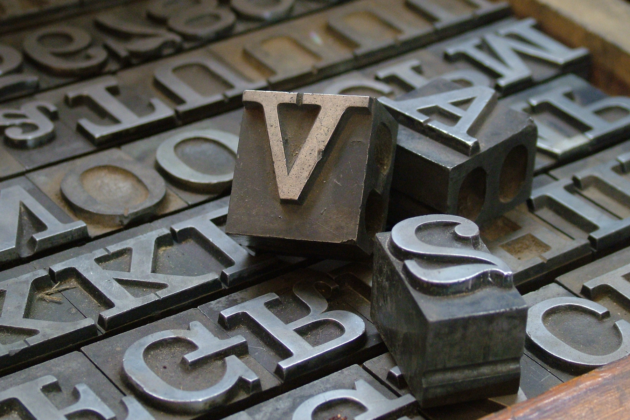
\includegraphics[width = 80mm]{fig/tipog}}
	{fonte}
	{label}
	{nota(s)}
	{legenda(s)}
\end{lstlisting}


\imagem{Titulo}{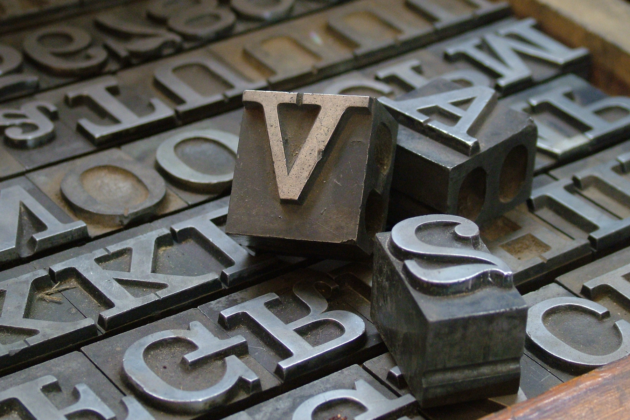
\includegraphics[width = 80mm]{fig/tipog}}{fonte}{label}{nota(s)}{legenda(s)}

Para fazer referência a esta figura é da mesma forma,\verb+\autoref{fig:label}+, \autoref{fig:label}

\subsection[Quadros e tabelas]{Quadros e tabelas}

Lembrando que quadros tem informações e são fechados lateralmente e verticalmente, tem a posição do título, fonte, nota e legenda diferentes da tabela.
\subsection[Quadros]{Inserir quadros}\label{ssec:quadros}

Para inserir um quadro são necessários 6 parâmetros:

\begin{lstlisting}
% ----------------------------------------------------------
%   Parametros
%    1 caption
%    2 elementos tabulados
%    3 fonte
%    4 qua:label
%    5 nota
%    6 legenda
\end{lstlisting}

Os elemento tabulados foram inseridos no ambiente tabular, com as laterais e parte superior e inferior fechados.

Este ambiente não quebra sua estrutura em páginas.

\begin{lstlisting}
\qquadro{Prefixos convencionados para referencias}
{\footnotesize
 \begin{tabular}{|l*{6}{|c}|}\hline
  \textbf{Elementos}:& 
       capitulos & secoes & 
       subsecoes & subsubsecoes &
       figuras   & imagens \\\hline
  \textbf{prefixos}:&
     cap &sec &
     ssec &sssec &
     fig & img\\\hline\hline
  \textbf{Elementos}:& tabelas &
     quadros & equacoes & exemplos &
     exercicios & questoes\\\hline	
  \textbf{prefixos}:&
     tab &    qua & 
     eq  &    exm & 
     exc &     que\\\hline\hline
  \textbf{Elementos}:& itens enumerados &
                       alineas&teoremas &
                       axiomas          & 
                       listagem         &\\\hline
  \textbf{prefixos}:&  inum & ali & teo & axi & lst &\\\hline
\end{tabular}}
{O autor(2021)}{quadrinho}{}{}
\end{lstlisting}

\qquadro{Prefixos convencionados para referencias}
{\footnotesize
 \begin{tabular}{|l*{6}{|c}|}\hline
  \textbf{Elementos}:& capítulos& 	seções&	subseções&	subsubseções&	
  figuras&	imagens \\\hline
  \textbf{prefixos}:&cap&sec&ssec&sssec&fig & img\\\hline\hline
  \textbf{Elementos}:&tabelas&	quadros&	
  equações& exemplos& exercícios & questões\\\hline	
  \textbf{prefixos}:&tab&qua&eq& exm & exc&que\\\hline\hline
  \textbf{Elementos}:&itens enumerados& alíneas&teoremas&	axiomas & listagem &\\\hline
  \textbf{prefixos}:&inum &ali&teo& axi &lst&\\\hline
\end{tabular}}
{O autor(2021)}{quadrinho}{}{}


A citação da fonte é feita por \verb+\citefig{bibkey}+.

Para fazer referência a este quadro, o comando \verb+\autoref{qua:quadrinho}+,\autoref{qua:quadrinho}


\subsection[Tabelas]{Inserir tabelas}

Para inserir uma tabela o comando é muito parecido, mas a normalização utilizada é o do IBGE na ABNT-UFPR.

\begin{lstlisting}
% simplificacao para colocar tabelas
% ----------------------------------------------------------
%   Parametros
%    1 caption
%    2 tabela
%    3 fonte
%    4 tab:label
%    5 nota
%    6 legenda


\tabela{T\'itulo do tabela}
{\begin{tabular}{r|c|c|c}\hline
		consumo & m\'edia & 
		m\'aximo & m\'inimo\\\hline
		& km/l& km/l& km/l\\\hline
		cidade & 11.5 & 14.8& 9.3 \\\hline
		estrada& 16.2 & 20.7& 13.4 \\\hline
\end{tabular}}
{\textcite{0230}}{exemplo}{Uma nota}{Uma legenda}
\end{lstlisting}


\tabela{T\'itulo do tabela}
{\begin{tabular}{r|c|c|c}\hline
		consumo & m\'edia & 
		m\'aximo & m\'inimo\\\hline
		& km/l& km/l& km/l\\\hline
		cidade & 11.5 & 14.8& 9.3 \\\hline
		estrada& 16.2 & 20.7& 13.4 \\\hline
\end{tabular}}
{\textcite{0230}}{exemplo}{Uma nota}{Uma legenda}


A citação da fonte é feita por \verb+\citefig{bibkey}+.

Para fazer referência a este quadro, o comando \verb+\autoref{tab:exemplo}+, \autoref{tab:exemplo}
\subsection[Equações]{Expressões matemáticas}

De preferencia ao uso do ambiente align:

\begin{lstlisting}
\begin{align}
 x + y &= 0\\
 x - y &= 2 \label{eq:2}
\end{align}
\end{lstlisting}


\begin{align}
x + y &= 0\\
x - y &= 2 \label{eq:2}
\end{align}

\subsection[Acronimos]{Siglas e símbolos}


\verb+\criarsimbolo{$\alpha$}{coeficiente de dilatação térmica}+ 

\criarsimbolo{$\alpha$}{coeficiente de dilatação térmica}, cria o símbolo e deixa anotado no texto;

\verb+\criarsigla{UFPR}{Universidade Federal do Paraná}+ 

\criarsigla{UFPR}{Universidade Federal do Paraná}\label{item:UFPR} apenas cria a sigla, sem deixar nada anotado no texto;

\verb+\criarsigla*{ABNT}{Associação Brasileira de Normas Técnicas}+ 

\criarsigla*{ABNT}{Associação Brasileira de Normas Técnicas} cria a sigla e deixa anotado no texto.

\subsection[Citações]{Citações e referências}

Para criar citações indiretas: Segundo \verb+\textcite{abntex2cite}+, \textcite{abntex2cite}.


Para citações diretas: "[...] tudo bem quando acaba bem."\cite{abntex2cite}. \verb+\cite{abntex2cite}+


\subsubsection{Criação de referencias citadas}

Para as citações feitas para serem empregadas no texto eu customizei a separação das referências bibliográficas através de \textit{keys}.


\subsubsection{Criação de referencias consultadas}

A criação de uma bibliografia consultada após o capítulo de referências do trabalho é feita para as referências que foram utilizadas com o \textit{key}= {consulta}:

\begin{lstlisting}
....
key={consultada},
....
\end{lstlisting}  


\subsubsection{Criação de referencias de documentos não publicados ou informais}

A criação de uma bibliografia consultada após o capítulo de referências do trabalho é feita para as referências que foram utilizadas com o \textit{key}= {npub-informal}:

\begin{lstlisting}
....
key={npub-informal},
....
\end{lstlisting}  

%%%%%%%%%%%%%%%%%%%%%%%%%%%%%%%%%%%%%%%%%%%%%%%%%%%%%%%%%%%%%%%%%

no arquivo referencias.bib, no manual ABNTeX2Modelo-glossario foi adicionado a key de consulta.

\begin{lstlisting}
@Manual{abntex2modelo-glossario,
	Title = {Exemplo de uso de gloss{\'a}rio com abnTeX2},
	Author      = {abnTeX2},
	Organization= {Equipe abnteX2},
	Year        = {2013},
	Bdsk-url-1  = {http://abntex2.googlecode.com/},
	Date-added  = {2013-03-11 13:38:46 +0000},
	Date-modified={2013-04-05 11:03:36 +0000},
	Url         = {http://abntex2.googlecode.com/},
	key         = {consulta},
}
\end{lstlisting}

adicionada a chave \textit{key}= = {consulta} para que ele seja mencionado na lista de obras consultadas.


\subsubsection{Para fazer referência às seções ou elementos enumerados}

\begin{lstlisting}
1. Capitulos: \verb+\autoref{cha:introd}+ 

2. Secoes: \verb+\autoref{sec:util}+ 

3. Subsecoes: \verb+\autoref{ssec:imafig}+

4. Imagens: \verb+\autoref{sssec:imagem}+ 

5. Apendices: \verb+\autoref{ap:primeiroAp}+ 
          
6. Anexos: \verb+\autoref{ax:primeiroAx}+ 
          
7. Equacoes: \verb+\autoref{eq:2}+

8. Itens enumerados \verb+\autoref{item:UFPR}+ 
	
\end{lstlisting}

\chapter{Introdução}

No ano de 2022 foram registrados 64.447 acidentes em rodovias federais, sendo o Paraná o terceiro estado com o maior número de acidentes ocorridos nestas rodovias \cite{AcidentesCNT}. A responsabilidade pela segurança viária nos mais de 75 mil quilômetros de rodovias e estradas federais é da Polícia Rodoviária Federal (PRF), instituição policial que, embora criada em 1928, foi integrada ao Sistema Nacional de Segurança Pública somente após o advento da Constituição Federal de 1988 \cite{InstitucionalPRF}.

\criarsigla{PRF}{Polícia Rodoviária Federal}

A PRF se faz presente em todos os estados brasileiros por meio de suas Unidades Administrativas e Operacionais. As Unidades Administrativas são compostas pela Unidade Central ou Sede, localizada em Brasília-DF, pelas Superintendências Regionais (SRPRF), localizadas em cada estado, e pelas Delegacias, situadas nos mais diversos municípios brasileiros. Sob responsabilidade das Delegacias estão os postos de fiscalização, conhecidos como Unidades Operacionais (UOP), distribuídos nas rodovias sob a circunscrição do órgão, proporcionando importante capilaridade nas ações da PRF \cite{CidadaoPRF}.

\criarsigla{SRPRF}{Superintendência Regional da PRF}
\criarsigla{UOP}{Unidade Operacional}

Acidentes ocorridos em rodovias federais podem ser registrados pelos próprios condutores de veículos envolvidos nos acidentes via internet ou presencialmente em uma UOP, desde que o acidente não seja caracterizado como relevante. Em caso de acidente relevante, o atendimento é iniciado com o recebimento da comunicação, em seguida a PRF se desloca até o local e prossegue com o levantamento dos dados e as demais providências necessárias, e finaliza o atendimento com a confecção de um Laudo Pericial de Acidente de Trânsito (LPAT) \cite{DATPRF, LPATPRF}. 

\criarsigla{LPAT}{Laudo Pericial de Acidente de Trânsito}

A PRF caracteriza um acidente como relevante quando pelo menos uma das situações ocorre:

\begin{itemize}
  \item Vítima lesionada ou morta;
  \item Danos a bens públicos não concedidos à iniciativa privada;
  \item Danos ao meio ambiente;
  \item Condutor inabilitado, com Carteira Nacional de Habilitação (CNH) suspensa ou cassada;
  \item Ocorrência de algum crime correlacionado diretamente ao acidente;
  \item Vazamento ou derramamento de produto perigoso;  
  \item Envolvimento de algum condutor sob influência de substância psicoativa de uso indevido;
  \item Interrupções totais ou parciais da via com grave prejuízo à fluidez;
  \item Ocorrência de incêndio ou submersão em algum dos veículos envolvidos \cite{UsuarioPRF}.
\end{itemize}

\criarsigla{CNH}{Carteira Nacional de Habilitação}

Atualmente há 378 UOPs em atividade em todo o território nacional \cite{UnidadesPRF}. Contudo, UOPs vêm sendo construídas, desativadas e reativadas de norte a sul do país ao longo dos anos (\autoref{fig:uops_evolution}). Decisões como estas implicam em consequências por longo período de tempo, o que torna essencial o uso de ferramentas de apoio à decisão para análise de alternativas. A distância entre as UOPs e os locais onde ocorrem os acidentes, além de impactar no tempo de resposta da PRF, também interfere diretamente no consumo de recursos públicos para suprir o uso de combustíveis, realizar a manutenção das viaturas, adquirir novas viaturas e equipamentos, replanejar o efetivo de servidores, entre outras necessidades.

\figura
{Quantidade de UOPs no Brasil ao longo dos anos}
{1}
{fig/uops_evolution.png}
{\textcite{ContasPRF2017}}
{uops_evolution}
{}
{}

Problemas envolvendo a decisão da localização de instalações, conhecidos na literatura como problema de localização de instalações, do inglês \textit{facility location problem} (FLP), há várias décadas atraem pesquisadores com foco tanto no setor privado (plantas industriais, bancos, instalações de varejo, etc.) como no setor público (hospitais, postos de serviços, etc.) \cite{Farahani2009}. 

\textcite{Dzator2017} discutiram a importância da aplicação de um modelo de p-Medianas para definir a localização de postos de emergência na cidade de Mackay, Austrália. \textcite{Cintrano2018} analisaram modelos de p-Medianas para determinar a localização ótima de estações de compartilhamento de bicicleta em Málaga, Espanha. \textcite{Wheeler2019}, por meio de uma aplicação de p-Medianas, demonstrou como áreas de patrulha policial em Carrollton (EUA) podem se tornar mais eficientes. \textcite{Zapata2020} utilizaram um modelo de p-Medianas para realocar armazéns de uma empresa da indústria automotiva. \textcite{Soares2021} desenvolveram uma ferramenta computacional baseada em um modelo de p-Medianas para apoiar a decisão da localização de Hospitais de Campanha para atendimento a pacientes com COVID-19. 

O problema de p-Medianas (PMP) é um FLP clássico que tem como intuito definir a localização de um conjunto de instalações para melhor servir um conjunto de pontos de demanda. Neste trabalho, a problemática será abordada com base no PMP.

\criarsigla{FLP}{Problema de localização de instalações}
\criarsigla{PMP}{Problema de p-Medianas}

\section{Objetivo Geral}

Este trabalho objetiva, por meio de modelo matemático, determinar o número e a localização das UOPs do estado do Paraná, de modo a minimizar as distâncias entre as UOPs e os locais dos acidentes.

\section{Objetivos Específicos}

Para atender ao objetivo geral, os objetivos específicos são:

\begin{itemize}
    \item Extrair os dados históricos de acidentes ocorridos nas rodovias do estado do Paraná;
    \item Transformar e tratar inconsistências nos dados;
    \item Formular e implementar computacionalmente o modelo matemático;
    \item Propor o número ideal de UOPs na rede;
    \item Propor a localização das UOPs considerando diferentes cenários;
    \item Propor uma sequência de expansão da rede de UOPs.
\end{itemize}

\section{Importância e Justificativa}

Eficiência é um dos princípios da Administração Pública do Brasil. De acordo com o artigo 37 da Constituição Federal: "A administração pública direta e indireta de qualquer dos Poderes da União, dos Estados, do Distrito Federal e dos Municípios obedecerá aos princípios de legalidade, impessoalidade, moralidade, publicidade e eficiência." \;\textcite{Brasil1988_gambiarra}. Segundo \textcite{Morais2009}, para obtenção dos resultados sociais aspirados pela sociedade, fazer uso dos recursos públicos com economia, zelo e dedicação não é suficiente, sendo necessário comprometimento político e institucional com um planejamento competente, de modo a oferecer serviços compatíveis com as necessidades da sociedade em extensão, qualidade e custos.

\textcite{Chan2012} definem eficiência dos gastos públicos como a capacidade do governo de maximizar suas atividades econômicas, dado um nível de gastos, ou minimizar suas despesas, dado um nível de atividade econômica. De acordo com \textcite{Izquierdo2018}, a eficiência do gasto público é essencial não só para a promoção do crescimento econômico de longo prazo, mas também para melhorar a equidade. Os autores também mencionam que o Brasil se destaca entre os países da América Latina pelo desperdício em gastos públicos ineficientes.

Assim sendo, este trabalho visa contribuir com a sociedade por meio de uma ferramenta com potencial para reduzir o consumo de recursos públicos, bem como elevar a qualidade do serviço prestado pela PRF à população, uma vez que a localização ótima das UOPs implica na redução do tempo de resposta da PRF nos atendimentos. Destaca-se que, embora o estudo limite-se ao estado do Paraná, a abordagem pode ser aplicada para os demais estados, bem como adaptada para para outras aplicações.

\section{Estrutura do Trabalho}

O presente trabalho está organizado em cinco capítulos. No primeiro é introduzido o tema do trabalho, bem como seus objetivos.

No segundo capítulo é feita uma fundamentação teórica, na qual são explicadas as características dos principais Problemas de Localização de Instalações, com ênfase no Problema de p-Medianas.

No terceiro capítulo é apresentada a metodologia utlizada no estudo, partindo do processo de data wrangling, clusterização dos pontos, formulação do modelo matemático até a geração das instâncias.

No quarto capítulo são analisados os resultados obtidos e apresentadas diferentes opções de solução.

Por fim, no quinto capítulo são realizadas as considerações finais e sugestões para trabalhos futuros.




% PARTE DA PREPARAÇÃO DA PESQUISA
% ----------------------------------------------------------
%\part{Preparação da pesquisa}
%\input{cap02}
%

% PARTE DOS REFERENCIAIS TEÓRICOS
% ----------------------------------------------------------
%\part{Referenciais teóricos}
%\input{cap03}
\chapter{Fundamentação Teórica}

Os Problemas de Localização de Instalações (FLPs) visam determinar a localização ideal de uma ou mais instalações para atender um conjunto de pontos de demanda. Em geral, os FLPs podem ser contínuos, ou seja, quando as instalações podem estar localizadas em qualquer lugar da região factível, ou discretos, que são os casos em que as instalações podem ser estabelecidas apenas em pontos candidatos \cite{Eiselt2011, AhmadiJavid2017}. O clássico problema de Weber, que visa determinar a localização de uma instalação minimizando os custos de produção e transporte \cite{Weber1909}, é um exemplo de FLP contínuo. Entretanto, as abordagens mais conhecidas estão associadas aos FLPs discretos, detalhados na \autoref{fig:flps_discretos}.

\figura
{Classificação dos problemas de localização discretos}
{1}
{fig/flps_discretos.png}
{\textcite{Daskin2008} e \textcite{AhmadiJavid2017}}
{flps_discretos}
{}
{}

Destaca-se que transformar um problema contínuo em discreto para resolvê-lo de maneira computacionalmente mais eficiente é uma prática conhecida.

\section{Problemas de cobertura}

Nos problemas de cobertura há um pressuposto de que os pontos de demanda devem estar há uma distância ou tempo máximo das instalações às quais foram alocados para serem considerados cobertos, por exemplo, por um serviço. No Problema de Cobertura de Conjunto, do inglês \textit{Set Covering Problem} (SCP), o objetivo é minimizar o número de instalações necessárias, dada uma distância ou tempo máximo de cobertura. Em contraste, o problema de p-Centros, do inglês \textit{p-Center Problem} (PCP), objetiva minimizar a distância ou tempo de cobertura, dado um conjunto de instalações. Em ambos os problemas todos os pontos de demanda devem ser cobertos, o que pode não ser viável em determinados contextos. Diante disso, uma alternativa é o Problema de Máxima Cobertura, do inglês \textit{Maximal Covering Problem} (MCP), que tem como objetivo maximizar o número de pontos de demanda atendidos, dado um numero fixo de instalações e uma distância ou tempo máximo de cobertura.

\criarsigla{SCP}{Problema de Cobertura de Conjunto}

\criarsigla{PCP}{Problema de p-Centros}

\criarsigla{MCP}{Problema de Máxima Cobertura}

\textcite{Vianna2019} discutiu a otimização do número e da localização de detectores de gás em plantas químicas como um SCP. Por meio dos resultados obtidos após testes realizados em dois casos reais de engenharia, o autor concluiu que a abordagem proposta é eficiente e viável. Já \textcite{Park2020} estudaram o desenvolvimento de um plano de voo para drones fornecerem rede \textit{wireless} em áreas de desastre. Após experimentos computacionais os autores concluíram que a abordagem proposta por meio de algoritmo exato é viável para áreas em escala realista com até 100 pontos de demanda e 2km de raio de cobertura.

\textcite{Lin2018} modelaram como um PCP a otimização da localização de postos de abastecimento de combustíveis alternativos, visando minimizar de forma equitativa os desvios de rota dos motoristas para realizar o reabastecimento. Os experimentos computacionais mostraram que podem existir diferentes soluções ótimas, mas elas estão associadas a diferentes distâncias totais de viagem. \textcite{Demange2020} discutiram a determinação da localização de abrigos em áreas florestais ameaçadas por incêndio como uma variação do PCP. Esta variacão considera a incerteza dos focos de incêndio e tem como objetivo minimizar a distância máxima de evacuação de qualquer zona (subdivisão do território em questão) até o abrigo mais próximo. Os autores concluíram por meio dos resultados dos experimentos que a abordagem é eficiente.

Em um projeto de rede de cadeia de suprimentos, \textcite{Rahmani2018} abordaram a definição do raio de cobertura dos centros de distribuição como um MCP. Dada a complexidade da combinação do MCP com outros requisitos da rede, os experimentos considerando um problema em larga escala, embora tenham gerado resultados com qualidade satisfatória, necessitaram de tempo relativamente alto para atingi-los. \textcite{Muren2020} propuseram uma variação do MCP para alocação de recursos de forma balanceada. Após testarem o modelo proposto no serviço de compartilhamento de bicicletas de uma grande cidade chinesa, os autores concluíram que a abordagem é geral o suficiente para ser aplicada em diversos problemas e economia compartilhada.

\section{Problemas de mediana}

\criarsigla{FCP}{Problema de Custo Fixo}

Nos problemas de mediana o intuito é definir a localização de um conjunto de instalações para melhor servir um conjunto de pontos de demanda. Enquanto nos problemas de cobertura há um foco mais individualizado nos pontos de demanda, nos problemas de mediana o objetivo é a minimização da distância média, normalmente ponderada pela demanda no ponto, entre os pontos de demanda e as instalações às quais foram alocados. A diferença fundamental entre o Problema de Custo Fixo, do inglês \textit{Fixed Charge Problem} (FCP) e o problema de p-Medianas , do inglês \textit{p-Median Problem} (PMP), é que o FCP objetiva minimizar o custo total de abertura das instalações, ao passo que o PMP desconsidera as diferenças entre os custos de abertura de cada instalação.

\textcite{Ghamami2015} modelaram a decisão da localização de carregadores de veículos elétricos nos estacionamentos existentes nos centros das cidades como um FCP. Os autores concluíram que o modelo proposto além de ser viável, introduz um mecanismo para que o nível de serviço possa ser compensado com o custo da infraestrutura. \textcite{Cheng2021} resolveram um FCP considerando incerteza na demanda e na disponibilidade da instalação. Os autores adotaram um estrutura de otimização robusta, em que, no primeiro estágio ocorre a decisão de localização e no segundo estágio a decisão de alocação, podendo ela ser adiada até que as informações de incerteza sejam reveladas. O algoritmo proposto foi comparado com um algoritmo de referência e os autores concluíram que a abordagem proposta é capaz de resolver mais instâncias em menor tempo.

\subsection{Problema de p-Medianas}

A formulação básica do PMP tem como objetivo encontrar a localização de $p$ instalações em uma rede, de modo que o custo total seja mínimo. O custo depende da distância entre o ponto de demanda $i$ e a instalação $j$, e da demanda no ponto $i$. \textcite{Jamshidi2009} menciona algumas suposições do PMP básico:

\begin{itemize}
  \item Relação linear entre custo e distância;
  \item Horizonte de tempo infinito;
  \item Capacidade infinita das instalações;
  \item Não considera custo inicial de setup;
  \item Demanda constante nos pontos;
  \item Instalações em localização fixa.
\end{itemize}

A seguir as notações utilizadas na formulação básica do PMP: \\

\hline
\textbf{Conjuntos:}

$I \colon \text{Conjunto de pontos de demanda,} \; I = \{1,2,\ldots,m\}\text{,}$

$J \colon \text{Conjunto de pontos candidatos,} \; J = \{1,2,\ldots,n\}\text{.}$ \\

\hline
\textbf{Parâmetros:}

$w_i \colon \text{Demanda no ponto }i \in I\text{,}$

$d_{ij} \colon \text{Distância do ponto de demanda }i \in I \text{ para o ponto candidato }j \in J \text{,}$

$p \colon \text{Número de instalações a serem estabelecidas,}$ \\

\hline
\textbf{Variáveis de decisão:}

$
    y_j \colon
    \begin{cases}
      1: & \text{se uma instalação é estabelecida no ponto candidato }j \in J \\
      0: & \text{caso contrário,}
    \end{cases}
$

$
    x_{ij} \colon
    \begin{cases}
      1: & \text{se o ponto de demanda }i \in I \text{ é associado à instalação }j \in J\\
      0: & \text{caso contrário.}
    \end{cases}
$ \\ \\

\hline

Em termos das notações apresentadas, o PMP é formulado da seguinte forma:

\begin{equation} \label{eq:fund_obj_function}
\text{min }Z = \sum\limits_{i \in I} \sum\limits_{j \in J} w_i d_{ij} x_{ij}.
\end{equation}

Sujeito a:

\begin{equation} \label{eq:fund_constraint1}
\sum\limits_{j \in J} x_{ij} = 1 \;\; \forall i \in I \text{,}
\end{equation}

\begin{equation} \label{eq:fund_constraint2}
\sum\limits_{j \in J} y_{j} = p \text{,}
\end{equation}

\begin{equation} \label{eq:fund_constraint3}
x_{ij} \leq y_j \;\; \forall i \in I \text{, }j \in J\text{,}
\end{equation}

\begin{equation} \label{eq:fund_constraint4}
x_{ij} \in \{0,1\} \;\; \forall i \in I \text{, }j \in J\text{,}
\end{equation}

\begin{equation} \label{eq:fund_constraint5}
y_j \in \{0,1\} \;\; \forall j \in J\text{.}
\end{equation}

Neste modelo, a função objetivo \ref{eq:fund_obj_function} minimiza a soma das distâncias ponderadas pela demanda. As restrições \ref{eq:fund_constraint1} garantem que cada ponto de demanda seja associado a somente uma instalação. A restrição \ref{eq:fund_constraint2} define o número total de instalações a serem estabelecidas na rede. As restrições \ref{eq:fund_constraint3} garantem que cada ponto de demanda seja associado a somente instalações abertas. As restrições \ref{eq:fund_constraint4} e \ref{eq:fund_constraint5} garantem o domínio das variáveis de decisão.

Modelos de p-Medianas podem ser resolvidos por métodos exatos ou aproximados. \textcite{Judecir2021} define os métodos exatos como métodos que garantem a solução ótima, desde que haja tempo e capacidade computacional suficientes. Já os métodos aproximados, segundo o autor, não garantem a otimalidade, mas geralmente encontram soluções factíveis satisfatórias em tempo consideravelmente menor com relação aos métodos exatos. Como exemplo de método exato podemos mencionar a Programação Linear Inteira Mista (PLIM). Quanto aos métodos aproximados, temos como exemplos os algoritmos heurísticos, metaheurísticos e de aprendizado por reforço.

\criarsigla{PLIM}{Programação Linear Inteira Mista}

\textcite{Nery2021} abordaram a determinação da localização de pontos apoio para veículos de auto socorro em Curitiba-PR como um PMP. Os autores discutiram possíveis cenários, a partir da resolução de uma série de modelos por meio de PLIM. \textcite{Wang2022} tiveram sucesso ao utilizarem um algoritmo de aprendizado por reforço para resolver o PMP em grande escala, com o objetivo de melhorar a performance com relação aos métodos aproximados tradicionalmente usados.

Por meio de um algoritmo heurístico, \textcite{Tang2020} resolveram um PMP para definir a localização de centros logísticos na cidade de Jinan, China. Os autores relataram que a solução encontrada atendeu os requisitos logísticos de uma distribuidora de frutas e vegetais. \textcite{Jnokov2017} propuseram o uso de um algoritmo metaheurístico combinado com PLIM para resolver grandes problemas de otimização combinatorial. A partir de experimentos com um PMP, os autores constataram que a abordagem proposta foi capaz de melhorar a FO em 6,4\%, em comparação com a abordagem tradicional testada.

\section{Outros problemas}

Os problemas que não se enquadram em alguma das principais categorias exibidas na \autoref{fig:flps_discretos} (Problemas de Cobertura e Problemas de Mediana) foram classificados por \textcite{Eiselt2011, AhmadiJavid2017} como outros problemas. Entre os problemas mais conhecidos desta categoria está o Problema de p-Dispersão, do inglês \textit{p-Dispersion Problem} (PDP), que tem como proposta maximizar a distância mínima de separação entre qualquer par de instalações em uma rede.

\criarsigla{PDP}{Problema de p-Dispersão}

\textcite{Sayyady2016} discutiram a otimização da localização de sensores de tráfego em uma malha rodoviária. No cenário descrito pelos autores, o problema foi abordado como um PDP devido ao limite do número de sensores disponíveis, e ao objetivo de maximizar a diversidade dos dados coletados. Os autores avaliaram uma  nova abordagem para resolver o problema e, por meio de experimentos, concluíram que a nova abordagem é mais eficiente do que os métodos exatos, pois permite resolver problemas maiores dentro de um tempo de execução razoável. Com a necessidade de satisfazer as restrições de distanciamento social impostas como medida de segurança contra a COVID-19, \textcite{Kudela2020} avaliou a determinação da localização de pessoas em local como um PDP. Com os resultados obtidos por meio de experimentos, o autor concluiu que a abordagem é viável no respectivo cenário.





% PARTE DA METODOLOGIA
% ----------------------------------------------------------
\chapter{Metodologia}

A metodologia utilizada consiste nas etapas exibidas na \autoref{fig:methodology_flow}. 

\figura
{Etapas da metodologia utilizada}
{1}
{fig/methodology/flow.png}
{O autor}
{methodology_flow}
{}
{}

Todas as etapas foram realizadas com apoio computacional por meio da linguagem de programação Python \cite{python}, utilizando principalmente as seguintes bibliotecas: Poetry \cite{poetry}, para garantir a reprodutibilidade do estudo; Pandas \cite{pandas}, para análise e manipulação dos dados; Numpy  \cite{numpy}, para operações com matrizes e vetores; Scikit-learn \cite{scikit-learn}, para análise de \textit{cluster}; Pyomo \cite{pyomo_book, pyomo_paper}, para formulação e resolução do modelo matemático em conjunto com o solver Gurobi \cite{gurobi}.

\section{Data Wrangling}

\textit{Data Wrangling} (DW) é um processo pelo qual os dados necessários são identificados, extraídos, limpos e integrados, de modo a produzir um conjunto de dados adequado para análise \cite{Furche2016}. Na \autoref{fig:methodology_dw_flow}, os retângulos representam as etapas de \textit{data wrangling} realizada neste estudo, enquanto os cilíndros informam a quantidade de registros após cada processamento.

\figura
{Etapas do processo de data wrangling}
{1}
{fig/methodology/dw_flow.png}
{O autor}
{methodology_dw_flow}
{}
{}

Os dados sobre acidentes foram extraídos da página eletrônica de dados abertos da PRF, que define dados abertos como dados institucionais acessíveis em formato legível por computador que qualquer pessoa usar e redistribuir de forma irrestrita \cite{DadosPRF}. O estudo considerou os acidentes ocorridos nas estradas e rodovias do Paraná entre os anos de 2018 e 2022. Portanto, foi necessário inicialmente concatenar os registros de cada ano e selecionar somente aqueles associados à SR do Paraná, formando um conjunto de dados composto por 37399 observações, em que cada observação corresponde a um acidente.

Foi feita uma validação inicial para garantir a qualidade dos dados, a qual consistiu na identificação e eliminação de registros incompletos ou com coordenadas geográficas inconsistentes, resultando em um conjunto de dados com 36745. Em função das coordenadas geográficas dos acidentes, foi feito, em seguida, um processo para garantir somente os registros ocorridos dentro do Paraná. O procedimento avaliou se cada ponto estava contido ou não no polígono composto pelos limites do estado do Paraná, e ao término o conjunto de dados foi reduzido para 36572 observações. 

Com o objetivo de identificar os pontos de acidentes inconsistentes com relação às delegacias aos quais estão associados, foi calculado o z-score (\autoref{eq:zscore}) sobre as coordenadas de latitude e longitude dos acidentes de cada delegacia. Os registros com o valor absoluto do z-score maior que 3 foram considerados outliers e, consequentemente, removidos, restando 36195 observações. 

\begin{equation} \label{eq:zscore}
z = \dfrac{x - \mu}{\sigma}
\end{equation}

Por meio do mapa disponibilizado na página de Unidades no site da PRF \cite{UnidadesPRF} foi extraído um arquivo do tipo kml com as informações geográficas das UOPs do Paraná. Foi feito um procedimento para transformar o kml em formato tabular, com o objetivo de acessar informações sobre as UOPs, em especial suas coordenadas geográficas. Para realizar o cruzamento com os dados dos acidentes foi necessário uma extensiva análise de geolocalização, uma vez que os códigos das UOPs presentes no conjunto de dados dos acidentes não correspondem ao identificador das UOPs do arquivo extraído. A \autoref{fig:methodology_accidents_uops_map} exibe a dispersão dos acidentes e das UOPs em todo o Paraná.

\figurah
{Dispersão dos acidentes e UOPs no estado do Paraná}
{1}
{fig/methodology/accidents_uops_map.png}
{O autor}
{methodology_accidents_uops_map}
{}
{}

Para viabilizar a solução exata e, ao mesmo tempo, garantir uma precisão aceitável, as coordenadas de latitude e longitude foram arredondadas para 1 casa decimal. Em seguida, as observações foram agregadas somando a quantidade de acidentes por quadrante (região de aproximadamente 11,1km ao redor do ponto após arredondamento), resultando em um novo conjunto de dados com 419 observações (\autoref{fig:methodology_accidents_agg_map}). 

\figurah
{Dispersão dos acidentes agrupados por quadrante}
{1}
{fig/methodology/accidents_agg_map.png}
{O autor}
{methodology_accidents_agg_map}
{}
{}

Cada quadrante recebeu um identificador único com base na seguinte regra: quando uma UOP está contida no quadrante, sua identificação é a da própria UOP fornecida pela PRF. Caso contrário, a identificação é composta pelo nome do município e um número sequencial.

\section{Clusterização dos pontos} \label{sec:clustering}

Com o objetivo de definir posteriormente a distância máxima que os quadrantes de acidentes poderão estar com relação às suas respectivas medianas, foi realizada uma análise de \textit{cluster} hierárquica aglomerativa em função da média mensal de acidentes nos quadrantes utilizando o método de Ward \cite{Ward1963}, um procedimento que tem como objetivo minimizar a variância intra-cluster. Neste tipo de análise, inicialmente cada observação é considerada um \textit{cluster} e gradualmente as observações são unidas, formando \textit{clusters} em função de uma medida de dissimilaridade, até restar um único \textit{cluster}. 

\figurah
{Dendrograma}
{1}
{fig/methodology/dendrogram.png}
{O autor}
{methodology_dendrogram}
{}
{}

Na \autoref{fig:methodology_dendrogram} é possível avaliar a formação gradativa dos \textit{clusters}. Neste gráfico conhecido como dendrograma, cada linha horizontal representa a ligação entre dois \textit{clusters} para a formação de um novo, enquanto as linhas verticais representam a dissimilaridade entre os \textit{clusters} formados, o que significa que quanto maior a linha horizontal, menos similares são os \textit{clusters}.

\tabela{Estatísticas da média mensal de acidentes por cluster}
{\begin{tabular}{l|c|c|c|c|c|c}\hline
    Cluster & Cont. & Média & D. Padr. & Mín. & Mediana & Máx.\\ \hline\hline
    Muito frequente & 1 & 33.92 & - & 33.92 & 33.92 & 33.92 \\
    Frequente & 5 & 18.49 & 3.15 & 13.61 & 20.08 & 21.26 \\
    Comum & 13 & 7.90 & 1.07 & 6.72 & 7.65 & 10.23 \\
    Incomum & 50 & 3.45 & 0.99 & 2.17 & 3.15 & 5.71 \\
    Raro & 80 & 1.35 & 0.30 & 0.93 & 1.25 & 2.06 \\
    Muito raro & 269 & 0.35 & 0.26 & 0.01 & 0.3 & 0.92 \\
    \hline
\end{tabular}}
{O autor}{methodology_cluster_stats}{}{}


Por meio de uma análise visual no dendrograma, foi decidido separar os quadrantes em 6 \textit{clusters}. A \autoref{tab:methodology_cluster_stats} exibe as estatísticas calculadas em função da média mensal de acidentes para cada um dos \textit{clusters}, e a \autoref{fig:methodology_accidents_cluster_map}, a dispersão dos quadrantes por \textit{cluster}.

\figurah
{Dispersão dos quadrantes por cluster}
{1}
{fig/methodology/accidents_cluster_map.png}
{O autor}
{methodology_accidents_cluster_map}
{}
{}

A primeira coluna da \autoref{tab:methodology_cluster_stats} exibe os nome de cada \textit{cluster}. Estes nomes foram definidos com base nestas estatísticas. O \textit{cluster} Muito raro, por exemplo, representa os 269 quadrantes com média inferior a 1 acidente por mês. Na outra extremidade temos o \textit{cluster} Muito frequente, que representa o único quadrante com média superior a 33 acidentes por mês.

\section{Formulação do modelo matemático}\label{sec:model_formulation}

A seguir estão as notações usadas na formulação do PMP: \\

\hline
\textbf{Conjuntos:}

$I \colon \text{Conjunto de quadrantes de acidentes,} \; I = \{1,2,\ldots,m\}\text{,}$

$V \colon \text{Conjunto de quadrantes candidatos a UOP,} \; V = \{1,2,\ldots,m\}\text{,}$

$U \colon \text{Conjunto de quadrantes com UOPs atuais,} \; U = \{m+1, m+2 \ldots, m + n\}\text{,}$

$J \colon V \cup U.$ \\

\hline
\textbf{Parâmetros:}

$w_i \colon \text{Histórico de acidente (demanda) no quadrante }i \in I\text{,}$

$d_{ij} \colon \text{Distância entre o quadrante de acidente }i \in I \text{ e o quadrante candidato a UOP }j \in J \text{,}$

$d_i^\text{max} \colon \text{Distância máxima que um quadrante de acidente }i \in I \text{ pode estar da UOP }j \in J\text{ ao qual é associado,}$

$p \colon \text{Número total de UOPs da rede,}$

$q \colon \text{Número mínimo de UOPs atuais a serem mantidas.}$ \\

\hline
\textbf{Variáveis de decisão:}

$
    y_j \colon
    \begin{cases}
      1: & \text{se uma UOP é instalada no quadrante candidato }j \in J \\
      0: & \text{caso contrário,}
    \end{cases}
$

$
    x_{ij} \colon
    \begin{cases}
      1: & \text{se o quadrante de acidente }i \in I \text{ é associado à UOP }j \in J\\
      0: & \text{caso contrário.}
    \end{cases}
$ \\ \\

\hline
\textbf{Formulação:}
\begin{equation} \label{eq:obj_function}
\text{Min. }Z = \sum\limits_{i \in I} \sum\limits_{j \in J} w_i d_{ij} x_{ij}.
\end{equation}

Sujeito a:

\begin{equation} \label{eq:constraint1}
\sum\limits_{j \in J} x_{ij} = 1 \;\; \forall i \in I \text{,}
\end{equation}

\begin{equation} \label{eq:constraint2}
\sum\limits_{j \in J} y_{j} = p \text{,}
\end{equation}

\begin{equation} \label{eq:constraint3}
\sum\limits_{u \in U} y_{u} \geq q \text{,}
\end{equation}

\begin{equation} \label{eq:constraint4}
x_{ij} \leq y_j \;\; \forall i \in I \text{; }j \in J\text{,}
\end{equation}

\begin{equation} \label{eq:constraint5}
d_{ij} x_{ij} \leq d_i^\text{max} \;\; \forall i \in I \text{; }j \in J\text{,}
\end{equation}

\begin{equation} \label{eq:constraint6}
x_{ij} \in \{0,1\} \;\; \forall i \in I \text{, }j \in J\text{,}
\end{equation}

\begin{equation} \label{eq:constraint7}
y_j \in \{0,1\} \;\; \forall j \in J\text{.}
\end{equation}

Neste modelo, a função objetivo \ref{eq:obj_function} minimiza a soma das distâncias ponderadas pela quantidade de acidentes. As restrições \ref{eq:constraint1} garantem que cada quadrante de acidente seja associado a somente uma UOP. A restrição \ref{eq:constraint2} define o número total de UOPs da rede. A restrição \ref{eq:constraint3} define o número mínimo de UOPs atuais a serem mantidas na rede. As restrições \ref{eq:constraint4} garantem que cada quadrante de acidente seja associado a somente UOPs instaladas. As restrições \ref{eq:constraint5} garantem que seja respeitada a distância máxima que um quadrante de acidente pode estar da UOP ao qual é associado. As restrições \ref{eq:constraint6} e \ref{eq:constraint7} garantem o domínio das variáveis de decisão.

\section{Criação da matriz de distâncias}

Para popular o parâmetro $d_{ij}$ exibido na \autoref{sec:model_formulation} foi necessário calcular a distância entre todos os pares de elementos dos conjuntos $I$ e $J$ e representá-las por meio de uma matriz de distâncias. O cálculo foi realizado por meio da fórmula de haversine (\autoref{eq:haversine}), utilizada para medir a distância entre dois pontos em uma esfera. Nesta expressão, $\theta$ e $\lambda$ representam, respectivamente, a latitude e longitude (em radianos) dos pontos, e $r = 6371$ é o raio da Terra em quilômetros \cite{Mahmoud2016}.

\begin{equation} \label{eq:haversine}
d = 2r \arcsen \sqrt{\sen^2 \left( \dfrac{\theta_2 - \theta_1}{2} \right) + \cos(\theta_1) \cos(\theta_2) \sen^2 \left( \dfrac{\lambda_2 - \lambda_1}{2}\right)} \text{.}
\end{equation} 

\section{Definição das distâncias máximas}

O objetivo desta etapa é a definição dos valores do parâmetro $d_i^\text{max}$ apresentado na \autoref{sec:model_formulation}.

\tabelah{Distâncias máximas entre quadrantes e UOPs}
{\begin{tabular}{l|c|c}\hline
    Cluster & Quadrantes & Dist. máxima (km) \\ \hline\hline
    Muito frequente & 1 & 60\\
    Frequente & 5 & 60\\
    Comum & 13 & 120\\
    Incomum & 50 & 120\\
    Raro & 80 & 180\\
    Muito raro & 269 & 180\\
    \hline
\end{tabular}}
{O autor}{methodology_dmax}{}{}

Após uma análise exploratória dados históricos dos acidentes, os valores foram defindos em função da segmentação realizada na \autoref{sec:clustering}, conforme exibido na \autoref{tab:methodology_dmax}.

\section{Criação e resolução das instâncias} \label{sec:instances}

Os parâmetros necessários para criação das instâncias do modelo formulado \autoref{sec:model_formulation} foram separados em dois grupos. O primeiro grupo é composto pelos parâmetros $w_i$, $d_{ij}$ e $d_i^{\text{max}}$, que são constantes em todas as instâncias. Já o segundo grupo, composto por $p$ e $q$, representam os parâmetros que serão variados em cada uma das instâncias. A partir do conjunto $R = \{P \times Q \mid q \leq p\}$, em que $P = \{1,2,3,\ldots,80\}$ e $Q = \{0,1,2,\ldots,33\}$, foram criadas 2192 instâncias, onde em cada instância os parâmetros $p$ e $q$ foram populados com os valores dos pares ordenados $(p,q)$ do conjunto $R$. Estas variações têm como objetivo a avaliação do impacto da FO.

Os dados de cada uma das instâncias resolvidas foram armazenados e serviram de insumo para a análise dos resultados discutida no \autoref{cha:results}.


% PARTE DOS RESULTADOS
% ----------------------------------------------------------
%\part{Resultados}
%\input{cap05}
\chapter{Resultados e Discussão} \label{cha:results}

\section{Soluções livres} \label{sec:solucoes_livres}

O conjunto $F = \{ (p,q) \in R \mid p \geq 5 \}$ representa as 2178 soluções factíveis encontradas nas execuções detalhadas na \autoref{sec:instances}. A \autoref{fig:plot_fo_q0} exibe a FO em função do parâmetro $p$, considerando somente as soluções livres (SL) representadas pelo conjunto $SL = \{ (p,q) \in F \mid q = 0 \}$. Para apoiar a interpretação do comportamento da FO, adicionou-se no gráfico o decrescimento percentual da FO (DPFO) a cada incremento em $p$. Neste gráfico observa-se que a partir de $p = 36$ a DPFO se estabiliza e cada incremento em $p$ passa a reduzir menos de 2,5\% da FO, indicando que o aumento no número de medianas não tem impacto significativo na redução do valor da FO.

\criarsigla{DPFO}{Decrescimento Percentual da FO}
\criarsigla{SL}{Solução livre}

\figurah
{FO em função do número de medianas a serem instaladas}
{1}
{fig/results/plot_fo_q0.png}
{O autor}
{plot_fo_q0}
{Soluções livres}
{}

Para a continuidade do estudo foram mantidas somente as SL em que $36 \leq p \leq 50$. Entre as 15 soluções que restaram, observou-se que 361 quadrantes (26 UOPs atuais e 335 UOPs candidatas) não foram escolhidos como mediana em qualquer das soluções. Dos 58 quadrantes que restaram, 29 foram escolhidos em todas as soluções, sendo 4 UOPs atuais e 25 UOPs candidatas (\autoref{tab:current_candidate_uops_aloc_q0}). Os 29 quadrantes restantes que foram escolhidos em somente parte das soluções, entre eles 3 UOPs atuais, são detalhados na \autoref{tab:uops_aloc_partial_q0}.

\tabela{UOPs escolhidas em todas as soluções}
{\begin{tabular}{l|l|l|l}\hline
      & UOP & Atual & Município \\ \hline\hline
    1 &               UOP06-DEL01-PR &   Sim &                Balsa Nova \\
    2 &               UOP05-DEL01-PR &   Sim &                 Paranaguá \\
    3 &               UOP02-DEL09-PR &   Sim &                 Paranavaí \\
    4 &               UOP01-DEL02-PR &   Sim &               Pato Branco \\
    5 &                 APUCARANA 01 &   Não &                 Apucarana \\
    6 &                 ARAPONGAS 03 &   Não &                 Arapongas \\
    7 &     CAMPINA GRANDE DO SUL 03 &   Não &     Campina Grande do Sul \\
    8 &     CAMPINA GRANDE DO SUL 06 &   Não &     Campina Grande do Sul \\
    9 &               CAMPO LARGO 04 &   Não &               Campo Largo \\
    10 &  CAPITAO LEONIDAS MARQUES 01 &   Não &  Capitão Leônidas Marques \\
    11 &                  CASCAVEL 04 &   Não &                  Cascavel \\
    12 &         CORNELIO PROCOPIO 02 &   Não &         Cornélio Procópio \\
    13 &                  CURITIBA 01 &   Não &                  Curitiba \\
    14 &                  CURITIBA 03 &   Não &                  Curitiba \\
    15 &                  CURITIBA 06 &   Não &                  Curitiba \\
    16 &             FOZ DO IGUACU 04 &   Não &             Foz do Iguaçu \\
    17 &                    IBAITI 01 &   Não &                    Ibaiti \\
    18 &                     IRATI 02 &   Não &                     Irati \\
    19 &               JACAREZINHO 01 &   Não &               Jacarezinho \\
    20 &                  LONDRINA 02 &   Não &                  Londrina \\
    21 &                   MARINGA 02 &   Não &                   Maringá \\
    22 &                MEDIANEIRA 01 &   Não &                Medianeira \\
    23 &                ORTIGUEIRA 08 &   Não &                Ortigueira \\
    24 &              PONTA GROSSA 06 &   Não &              Ponta Grossa \\
    25 & SANTO ANTONIO DO SUDOESTE 02 &   Não & Santo Antônio do Sudoeste \\
    26 &      SAO JOSE DOS PINHAIS 03 &   Não &      São José dos Pinhais \\
    27 &      SAO JOSE DOS PINHAIS 06 &   Não &      São José dos Pinhais \\
    28 &         SAO MATEUS DO SUL 05 &   Não &         São Mateus do Sul \\
    29 &          UNIAO DA VITORIA 02 &   Não &          União da Vitória \\
 \hline
\end{tabular}}
{O autor}{current_candidate_uops_aloc_q0}{}{}

A \autoref{fig:plot_sols_q0_partial_uops} exibe a alocação de cada uma das UOPs da \autoref{tab:uops_aloc_partial_q0}. Nela, observa-se que a transição da SL com 36 para 37 medianas ocorre com a instalação da UOP MANDIRITUBA 02. Já a transição para a solução com 38 medianas depende da desinstalação de FAROL 02 e instalação de CAMPO MOURAO 02 e UBIRATA 04. Por fim, a transição para a solução com 39 medianas ocorre com a desinstalação de CANTAGALO 01 e GUARAPUAVA 08, e instalação de GUARAPUAVA 03, PRUDENTOPOLIS 02 e VIRMOND 01. 

\figurah
{Alocações nas soluções livres}
{1}
{fig/results/plot_sols_q0_partial_uops.png}
{O autor}
{plot_sols_q0_partial_uops}
{Desconsideradas as UOPs alocadas em todas as soluções}
{}

Percebe-se que, com exceção da transição para a SL com 37 medianas, não é possível fazer uma simples adição de UOP na rede e ainda mantê-la otimizada, o que pode não ser financeiramente viável. Entretanto, a situação muda quando observamos a solução livre com 39 medianas. Neste caso, para acrescentar mais 1 UOP na rede, basta instalar MORRETES 02. E, observando novamente a \autoref{fig:plot_sols_q0_partial_uops}, percebe-se que é possível expandir a rede até 42 UOPs por meio de simples adições. 

\tabelah{UOPs escolhidas em parte das soluções}
{\begin{tabular}{l|l|l|l|c}\hline
   & UOP  & Atual  &  Município & Soluções \\ \hline\hline
 1 &             UOP04-DEL01-PR &   Sim &               Guaratuba & 12 (80\%) \\
 2 &             UOP02-DEL06-PR &   Sim & Marechal Cândido Rondon &  8 (53\%) \\
 3 &             UOP01-DEL04-PR &   Sim &                Cascavel &  2 (13\%) \\ \hline
 4 &             MANDIRITUBA 02 &   Não &             Mandirituba & 14 (93\%) \\
 5 &            CAMPO MOURAO 02 &   Não &            Campo Mourão & 13 (87\%) \\
 6 &                 UBIRATA 04 &   Não &                 Ubiratã & 13 (87\%) \\
 7 &              GUARAPUAVA 03 &   Não &              Guarapuava & 12 (80\%) \\
 8 &           PRUDENTOPOLIS 02 &   Não &           Prudentópolis & 12 (80\%) \\
 9 &                MORRETES 02 &   Não &                Morretes & 11 (73\%) \\
10 &                MARIALVA 01 &   Não &                Marialva & 10 (67\%) \\
11 &              GUARANIACU 01 &   Não &              Guaraniaçu &  9 (60\%) \\
12 &                 MARINGA 01 &   Não &                 Maringá &  9 (60\%) \\
13 &                  GUAIRA 03 &   Não &                  Guaíra &  8 (53\%) \\
14 &                  TIBAGI 04 &   Não &                  Tibagi &  8 (53\%) \\
15 &                   IMBAU 02 &   Não &                   Imbaú &  7 (47\%) \\
16 & MARECHAL CANDIDO RONDON 04 &   Não & Marechal Cândido Rondon &  7 (47\%) \\
17 &                  TIBAGI 03 &   Não &                  Tibagi &  7 (47\%) \\
18 &                  CANDOI 05 &   Não &                  Candói &  6 (40\%) \\
19 &              GUARANIACU 02 &   Não &              Guaraniaçu &  6 (40\%) \\
20 &        NOVA LARANJEIRAS 02 &   Não &        Nova Laranjeiras &  6 (40\%) \\
21 &                 VIRMOND 01 &   Não &                 Virmond &  6 (40\%) \\
22 &                LONDRINA 03 &   Não &                Londrina &  5 (33\%) \\
23 &                PALMEIRA 07 &   Não &                Palmeira &  4 (27\%) \\
24 &               CANTAGALO 01 &   Não &               Cantagalo &  3 (20\%) \\
25 &              GUARAPUAVA 08 &   Não &              Guarapuava &  3 (20\%) \\
26 &               GUARATUBA 03 &   Não &               Guaratuba &  3 (20\%) \\
27 &          TIJUCAS DO SUL 03 &   Não &          Tijucas do Sul &  3 (20\%) \\
28 &                   FAROL 02 &   Não &                   Farol &  2 (13\%) \\
29 &                CURITIBA 04 &   Não &                Curitiba &   1 (7\%) \\
 \hline
\end{tabular}}
{O autor}{uops_aloc_partial_q0}{}{}

Portanto, foi assumido neste momento que 39 é o número ideal de UOPs para a rede. A \autoref{fig:results_plot_map_sl39} ilustra a dispersão das UOPs na solução livre com 39 medianas (SL39).

\figurah
{Dispersão das UOPs na solução livre com 39 medianas}
{1}
{fig/results/plot_map_sl39.png}
{O autor}
{results_plot_map_sl39}
{}
{}

Ja a tabela \autoref{tab:results_uops_table_sl39} exibe a lista das UOPs alocadas na SL 39.

\tabelah{UOPs alocadas na solução livre com 39 medianas}
{\begin{tabular}{l|l|l|l}\hline
   & UOP  & Atual  &  Município \\ \hline\hline
 1 &               UOP01-DEL02-PR &   Sim &               Pato Branco \\
 2 &               UOP02-DEL09-PR &   Sim &                 Paranavaí \\
 3 &               UOP04-DEL01-PR &   Sim &                 Guaratuba \\
 4 &               UOP05-DEL01-PR &   Sim &                 Paranaguá \\
 5 &               UOP06-DEL01-PR &   Sim &                Balsa Nova \\ \hline
 6 &                 APUCARANA 01 &   Não &                 Apucarana \\
 7 &                 ARAPONGAS 03 &   Não &                 Arapongas \\
 8 &     CAMPINA GRANDE DO SUL 03 &   Não &     Campina Grande do Sul \\
 9 &     CAMPINA GRANDE DO SUL 06 &   Não &     Campina Grande do Sul \\
10 &               CAMPO LARGO 04 &   Não &               Campo Largo \\
11 &              CAMPO MOURAO 02 &   Não &              Campo Mourão \\
12 &  CAPITAO LEONIDAS MARQUES 01 &   Não &  Capitão Leônidas Marques \\
13 &                  CASCAVEL 04 &   Não &                  Cascavel \\
14 &         CORNELIO PROCOPIO 02 &   Não &         Cornélio Procópio \\
15 &                  CURITIBA 01 &   Não &                  Curitiba \\
16 &                  CURITIBA 03 &   Não &                  Curitiba \\
17 &                  CURITIBA 06 &   Não &                  Curitiba \\
18 &             FOZ DO IGUACU 04 &   Não &             Foz do Iguaçu \\
19 &                GUARANIACU 01 &   Não &                Guaraniaçu \\
20 &                GUARAPUAVA 03 &   Não &                Guarapuava \\
21 &                    IBAITI 01 &   Não &                    Ibaiti \\
22 &                     IRATI 02 &   Não &                     Irati \\
23 &               JACAREZINHO 01 &   Não &               Jacarezinho \\
24 &                  LONDRINA 02 &   Não &                  Londrina \\
25 &               MANDIRITUBA 02 &   Não &               Mandirituba \\
26 &   MARECHAL CANDIDO RONDON 04 &   Não &   Marechal Cândido Rondon \\
27 &                   MARINGA 02 &   Não &                   Maringá \\
28 &                MEDIANEIRA 01 &   Não &                Medianeira \\
29 &                ORTIGUEIRA 08 &   Não &                Ortigueira \\
30 &              PONTA GROSSA 06 &   Não &              Ponta Grossa \\
31 &             PRUDENTOPOLIS 02 &   Não &             Prudentópolis \\
32 & SANTO ANTONIO DO SUDOESTE 02 &   Não & Santo Antônio do Sudoeste \\
33 &      SAO JOSE DOS PINHAIS 03 &   Não &      São José dos Pinhais \\
34 &      SAO JOSE DOS PINHAIS 06 &   Não &      São José dos Pinhais \\
35 &         SAO MATEUS DO SUL 05 &   Não &         São Mateus do Sul \\
36 &                    TIBAGI 04 &   Não &                    Tibagi \\
37 &                   UBIRATA 04 &   Não &                   Ubiratã \\
38 &          UNIAO DA VITORIA 02 &   Não &          União da Vitória \\
39 &                   VIRMOND 01 &   Não &                   Virmond \\
 \hline
\end{tabular}}
{O autor}{results_uops_table_sl39}{}{}

\criarsigla{SL39}{Solução livre com 39 medianas}

\subsection{Expansão da rede partindo da SL39} \label{ssec:expansao_sl39}

Ao avaliar a \autoref{fig:plot_sols_q0_partial_uops}, foi percebido que é possível expandir a rede, partindo da SL39, até 42 UOPs por meio de simples adições. Entretanto, para expandir a rede para 43 UOPs torna-se necessário desinstalar MARECHAL CANDIDO RONDON 04, e instalar GUAIRA 03 e UOP02-DEL06-PR. Contudo, uma vez que a distância entre os quadrantes MARECHAL CANDIDO RONDON 04 e UOP02-DEL06-PR é de aproximadamente 11km, foi observado que, por um custo de 0,51\% na FO, é possível manter MARECHAL CANDIDO RONDON 04 na solução, incluindo apenas GUAIRA 03. 

\tabelah{Impacto da realocação das UOPs}
{\begin{tabular}{c|l|l|c|c}\hline
 Rede ($p$) & UOP (de) & UOP (para) & Dist. & Impacto FO \\ \hline\hline
 43 & UOP02-DEL06-PR & MAL CAND RONDON 04 & 11 km & +0,51\% \\
 44 & TIBAGI 03 & TIBAGI 04 & 15 km & +0,93\% \\
 45 & GUARANIACU 02 & GUARANIACU 01 & 23 km & +1,12\% \\
 45 & CANDOI 05 & VIRMOND 01 & 15 km & +0,69\% \\
 48 & GUARATUBA 03 & UOP04-DEL01-PR & 10 km & +0,30\% \\
 \hline
\end{tabular}}
{O autor}{uops_aloc_q0}{}{}

A \autoref{tab:uops_aloc_q0}, exibe esta e as demais realocações necessárias para expansão da rede até 50 UOPs, por meio de simples adições na rede, bem como os respectivos impactos na FO. 

\tabelah{Expansão da solução livre com 39 medianas}
{\begin{tabular}{c|l|l|l}\hline
 Rede ($p$) & UOP a incluir & Atual & Município \\ \hline\hline
 40 &         MORRETES 02 &   Não &         Morretes \\
  41 &         MARIALVA 01 &   Não &         Marialva \\
  42 &          MARINGA 01 &   Não &          Maringá \\
  43 &           GUAIRA 03 &   Não &           Guaíra \\
  44 &            IMBAU 02 &   Não &            Imbaú \\
  45 & NOVA LARANJEIRAS 02 &   Não & Nova Laranjeiras \\
  46 &         LONDRINA 03 &   Não &         Londrina \\
  47 &         PALMEIRA 07 &   Não &         Palmeira \\
  48 &   TIJUCAS DO SUL 03 &   Não &   Tijucas do Sul \\
  49 &      UOP01-DEL04-PR &   Sim &         Cascavel \\
  50 &         CURITIBA 04 &   Não &         Curitiba \\
 \hline
\end{tabular}}
{O autor}{uops_expansion_q0}{}{}

E, por fim, a \autoref{tab:uops_expansion_q0} exibe o plano de expansão da SL39 até 50 medianas.

\section{Soluções restritas}

Considerando as soluções restritas (SR) representadas pelo conjunto $SR = \{ (p,q) \in F \mid p = 39 \text{ e } q > 0 \}$, de maneira análoga ao gráfico da \autoref{fig:plot_fo_q0}, a \autoref{fig:plot_fo_p39} exibe a FO em função do parâmetro $q$. Observa-se no gráfico que a partir de $q = 15$ a DPFO se estabiliza e cada decremento em $q$ passa a reduzir menos de 0,25\% da FO, indicando que a partir deste ponto desobrigar o modelo a manter UOPs atuais na solução não impacta significativamente na redução do valor da FO.

\figurah
{FO em função do número mínimo de UOPs a serem mantidas}
{1}
{fig/results/plot_fo_p39.png}
{O autor}
{plot_fo_p39}
{Soluções restritas com 39 medianas.}
{}

A solução restrita com 15 UOPs atuais (SR15) apresentou o valor de 383230 na FO, ao passo que o valor da FO da SL39 é de 378908. Nesta comparação observa-se que pelo custo de 1,15\% no valor da FO, é possível fixar 15 UOPs atuais na solução com 39 medianas. A \autoref{fig:results_plot_map_sr15} ilustra as dispersão das UOPs na SR15.

\figurah
{Dispersão das UOPs na solução com 39 medianas e 15 UOPs atuais}
{1}
{fig/results/plot_map_sr15.png}
{O autor}
{results_plot_map_sr15}
{}
{}

Ja a tabela \autoref{tab:results_uops_table_sr15} exibe as substituições necessárias na SL39 (\autoref{tab:results_uops_table_sl39}) para transformar na SR15.

\tabelah{Substituições necessárias de SL39 para SR15}
{\begin{tabular}{l|l|l|l}\hline
   & UOP (de)  & UOP (para)  &  Dist. \\ \hline\hline
 1 &         SAO MATEUS DO SUL 05 & UOP03-DEL07-PR &  10 km \\
 2 &                   VIRMOND 01 &   CANTAGALO 01 &  10 km \\
 3 &              CAMPO MOURAO 02 & UOP01-DEL09-PR &  10  km \\
 4 &                    TIBAGI 04 & UOP03-DEL09-PR &  11km \\
 5 &   MARECHAL CANDIDO RONDON 04 & UOP02-DEL06-PR &  11 km \\
 6 & SANTO ANTONIO DO SUDOESTE 02 & UOP03-DEL04-PR &  15 km \\
 7 &                   UBIRATA 04 & UOP04-DEL02-PR &  15 km \\
 8 &                GUARAPUAVA 03 & UOP02-DEL03-PR &  20 km \\
 9 &          UNIAO DA VITORIA 02 &    BARRACAO 04 &  23 km \\
10 &                 APUCARANA 01 & UOP01-DEL08-PR &  23 km \\
11 &  CAPITAO LEONIDAS MARQUES 01 & UOP02-DEL02-PR &  30 km \\
12 &             PRUDENTOPOLIS 02 & UOP03-DEL02-PR & 192 km  \\
 \hline
\end{tabular}}
{O autor}{results_uops_table_sr15}{}{}

\criarsigla{SR}{Solução restrita}
\criarsigla{SR15}{Solução restrita com 15 UOPs atuais}

\subsection{Expansão da rede partindo da SR15}

A \autoref{fig:plot_sols_q15_p39_partial_uops} exibe a alocação das UOPs da SR15 até a solução com 50 medianas, desprezando as UOPs alocadas em todas as soluções nesta faixa selecionada. Nela, observa-se que a transição de 40 para 41 medianas depende da desinstalação de CANTAGALO 01, UOP01-DEL08-PR e MORRETES 02, e a instalação de UOP01-DEL06-PR, GUARAPUAVA 03, PRUDENTOPOLIS 02 e VIRMOND 01. Além disso, nota-se que a MORRETES 02 volta a ser alocada na solução com 42 medianas. 

\figurah
{Alocações nas soluções restritas com 15 UOPs atuais}
{1}
{fig/results/plot_sols_q15_p39_partial_uops.png}
{O autor}
{plot_sols_q15_p39_partial_uops}
{Desconsideradas as UOPs alocadas em todas as soluções}
{}

Com o intuito de reduzir o número de desinstalações necessárias durante o aumento do número de medianas, foram propostas as realocações exibidas na \autoref{tab:uops_aloc_q15_p39}, baseadas na abordagem realizada em \autoref{ssec:expansao_sl39}.

\tabelah{Impacto da realocação das UOPs na solução restrita com 15 UOPs atuais}
{\begin{tabular}{c|l|l|c|c}\hline
 Rede ($p$) & UOP (de) & UOP (para) & Dist. & Impacto FO \\ \hline\hline
 41 & PRUDENTOPOLIS 02 & MORRETES 02 & 233 km & +20\% \\
 41 & VIRMOND 01 & CANTAGALO 01 & 10 km & +0,01\% \\
 41 & GUARAPUAVA 03 & UOP01-DEL08-PR & 20 km & +1,3\% \\
 41 & GUARANIACU 02 & GUARANIACU 01 & 23 km & +0,86\% \\
 44 & UNIAO DA VITORIA 01 & UOP03-DEL02-PR & 15 km & +0,31\% \\
 44 & CANDOI 05 & CANTAGALO 01 & 23 km & +1,03\% \\
 47 & CAPITAO LEONIDAS MARQUES 01 & UOP02-DEL02-PR & 30 km & +0,95\% \\
 47 & SANTO ANTONIO DO SUDOESTE 02 & BARRACAO 04 & 15 km & +0,29\% \\
 48 & IMBAU 02 & UOP02-DEL03-PR & 15 km & +0,59\% \\
 49 & UBIRATA 04 & UOP03-DEL04-PR & 15 km & +0,01\% \\
 50 & GUARATUBA 03 & UOP04-DEL01-PR & 10 km & +0,31\% \\
 \hline
\end{tabular}}
{O autor}{uops_aloc_q15_p39}{}{}

A \autoref{tab:uops_expansion_q15} exibe o plano de expansão da SR15 até 50 medianas.

\tabelah{Expansão da solução restrita com 15 UOPs atuais}
{\begin{tabular}{c|l|l|l}\hline
 Rede ($p$) & UOP a incluir & Atual & Município \\ \hline\hline
 40 &       MORRETES 02 &   Não &           Morretes \\
  41 &    UOP01-DEL06-PR &   Sim &             Guaíra \\
  42 &  PRUDENTOPOLIS 02 &   Não &      Prudentópolis \\
  43 &        MARINGA 01 &   Não &            Maringá \\
  44 &    UOP02-DEL04-PR &   Sim & Laranjeiras do Sul \\
  45 &       LONDRINA 03 &   Não &           Londrina \\
  46 &       PALMEIRA 07 &   Não &           Palmeira \\
  47 &    UOP01-DEL04-PR &   Sim &           Cascavel \\
  48 &         TIBAGI 03 &   Não &             Tibagi \\
  49 &    UOP04-DEL04-PR &   Sim &          Lindoeste \\
  50 & TIJUCAS DO SUL 03 &   Não &     Tijucas do Sul \\
 \hline
\end{tabular}}
{O autor}{uops_expansion_q15}{}{}

\section{Soluções atuais}

Com o objetivo de avaliar a rede atual de UOPs, gerou-se o conjunto de soluções atuais (SA) $SA = \{ (p,q) \in F \mid p = q \}$ e a partir dele foi gerado o gráfico da \autoref{fig:results_plot_fo_q33}. Neste gráfico observa-se que a partir de $p = 30$ cada incremento em $p$ passa a reduzir menos de 1\% da FO.

\criarsigla{SA}{Solução atual}

\figurah
{FO em função do número de medianas a serem instaladas}
{1}
{fig/results/plot_fo_q33.png}
{O autor}
{results_plot_fo_q33}
{Soluções considerando somente UOPs atuais}
{}

A solução atual com 29 UOPs atuais (SA29) apresentou o valor de 677026 na FO, enquanto o valor da FO da solução atual com 33 UOPs (SA33) é de 664280. Nesta comparação observa-se que por um custo de 1,92\% da FO seria possível desativar as 4 UOPs listadas na \autoref{tab:uops_q33_to_remove}.

\criarsigla{SA29}{Solução atual com 29 UOPs}
\criarsigla{SA33}{Solução atual com 33 UOPs}

\tabelah{UOPs atuais com possibilidade de desativação}
{\begin{tabular}{l|l|l}\hline
   & UOP  &  Município \\ \hline\hline
1 & UOP03-DEL06-PR &              Alto Paraíso \\
2 & UOP04-DEL05-PR &             Foz do Iguaçu \\
3 & UOP04-DEL04-PR &                 Lindoeste \\
4 & UOP01-DEL05-PR & Santa Terezinha de Itaipu \\
 \hline
\end{tabular}}
{O autor}{uops_q33_to_remove}{}{}

Considerando um cenário em que todas as 33 UOPs atuais são aproveitadas em uma solução com 39 medianas, para atingir o número de medianas seria necessário adicionar as UOPs listadas na \autoref{tab:uops_q33_to_add}

\tabelah{UOPs a serem adicionadas na solução com 33 UOPs atuais}
{\begin{tabular}{l|l|l}\hline
   & UOP  &  Município \\ \hline\hline
1 &                 CAMBE 01 &                 Cambé \\
2 & CAMPINA GRANDE DO SUL 06 & Campina Grande do Sul \\
3 &              CURITIBA 01 &              Curitiba \\
4 &              CURITIBA 03 &              Curitiba \\
5 &              CURITIBA 06 &              Curitiba \\
6 &               MARINGA 02 &               Maringá \\
 \hline
\end{tabular}}
{O autor}{uops_q33_to_add}{}{}

A \autoref{fig:results_plot_map_p39_q33} ilustra as alocações da SA33, considerando as inclusões listadas na \autoref{tab:uops_q33_to_add}.

\figurah
{Solução atual com 33 UOPs}
{1}
{fig/results/plot_map_p39_q33.png}
{O autor}
{results_plot_map_p39_q33}
{}
{}



% Finaliza a parte no bookmark do PDF
% para que se inicie o bookmark na raiz
% e adiciona espaço de parte no Sumário
% ----------------------------------------------------------
%\phantompart

% ---
% Conclusão (outro exemplo de capítulo sem numeração e presente no sumário)
% ---
%\chapter*[Conclusão]{Conclusão}
%\addcontentsline{toc}{chapter}{Conclusão}
% ---
%\input{cap06}
\chapter{Considerações Finais}

Uma vez que a problemática da distribuição eficiente dos postos de fiscalização (UOP) da Polícia Rodoviária Federal (PRF) afeta diretamente o consumo de recursos públicos e a qualidade do serviço prestado pela PRF à população, esta dissertação buscou, com uma abordagem baseada no problema de p-Medianas, determinar o número e a localização das UOPs no estado do Paraná, com o objetivo de minimizar as distâncias entre as UOPs e os locais com registros de acidentes.

No primeiro cenário, dentre os quatro avaliados durante o estudo, o objetivo foi encontrar o número e a localização das UOPs entre todas as possíveis localizações mapeadas. Nesta etapa foi concluído que 39 seria o número ideal de UOPs e que 5 das UOPs já existentes poderiam ser aproveitadas na rede. Além disso, foi definida uma sequência de expansão da rede até 50 UOPs com o objetivo de minimizar o impacto financeiro e operacional quando houver necessidade de adicionar novos postos. Em termos práticos esta abordagem prescreve a desativação de 28 UOPs e a construção de outras 34 unidades, mas a solução proposta não foi considerada no estudo como viável, dado o alto investimento necessário e o risco do comportamento dos acidentes no período analisado não se manter no futuro. 

Já no segundo cenário, considerando o número de UOPs definido no cenário anterior, o objetivo foi encontrar o número máximo de UOPs já existentes com o mínimo impacto na função objetivo (FO). Nesta etapa foi concluído que, com um custo de 1,15\% na FO do primeiro cenário, é possível fixar 15 das 33 UOPs já existentes na solução. Assim como no primeiro cenário, também foi definida uma sequência para expansão da rede até 50 UOPs. Em termos práticos esta abordagem prescreve a desativação de 18 UOPs e a construção de outras 24, mas pelos mesmos motivos alegados no cenário 1, a solução proposta não foi considerada viável. Entretanto, é possível que em outra UF a abordagem resulte em uma prescrição viável.

O terceiro e quarto cenário consideraram a rede com as 33 UOPs já existentes. No cenário 3, que teve como objetivo avaliar a possibilidade de reduzir o número de UOPs, foi concluído que, com um custo de 1,92\% na FO, é possível reduzir o número de UOPs da rede para 29. Na prática esta solução além de mitigar os custos para manter em funcionamento as 4 UOPs eleitas para serem desativadas, ela permite remanejar o efetivo para outras atribuições, podendo inclusive, mediante estudo futuro, serem aproveitados em postos móveis localizados conforme a demanda. Já no cenário 4, que teve como objetivo expandir a rede atual para o número de 39 UOPs definido no primeiro cenário, obteve-se em ordem sequencial as 6 UOPs a serem construídas.

A abordagem baseada no problema de p-Medianas se demonstrou sensível ao valor de $p$ escolhido, fazendo-se necessária a análise e o ajuste da solução em determinados cenários para viabilizar a expansão da rede com o menor impacto financeiro e operacional possível. Por outro lado, a possibilidade de escolher diferentes valores de $p$ permitiu a análise de diferentes cenários, trazendo flexibilidade a esta abordagem determinística ao oferecer para o tomador de decisão um leque de possibilidades. Além disso, há o risco do modelo de p-Medianas simplificar excessivamente o problema de geolocalização e, consequentemente, gerar soluções otimizadas do ponto de vista matemático, mas que podem não ser alinhadas com as necessidades operacionais da PRF. No entanto, a abordagem permite a incorporação de restrições específicas para alinhar as soluções com as necessidades operacionais da PRF.

Cinco próximos passos foram mapeados com o intuito de aumentar a robustez dos resultados obtidos: o primeiro deles é a realização de um levantamento junto à PRF sobre possíveis regras para a localização e distância entre UOPs e incluí-las como restrições nos modelos. O segundo passo é considerar nos modelos o efetivo de servidores por UOP, informação que também depende de um levantamento junto à PRF. O terceiro passo é substituir as distâncias calculadas por meio da fórmula de Haversine pelas distâncias reais extraídas via API do Google Maps ou algum outro serviço de geolocalização. O quarto passo é agregar os acidentes considerando coordenadas mais precisas, o que, consequentemente, aumentaria o número de quadrantes. E, por fim, o quinto passo é considerar como parâmetro nos modelos os resultados de um modelo de previsão de acidentes ao invés dos dados históricos.




% ELEMENTOS PÓS-TEXTUAIS
% ----------------------------------------------------------
\postextual

% Ajuste vertical do titulo de referencias no sumário
% ----------------------------------------------------------
\addtocontents{toc}{\vspace{-6pt}}

% Referências bibliográficas
% ----------------------------------------------------------
%\bibliography{referencias}

\begingroup

\printbibliography[heading=bay,notkeyword= {consulta}, notkeyword={npub-informal}]

\printbibliography [keyword= consulta, title = FONTES DE CONSULTA]
\endgroup

% ----------------------------------------------------------

% Ajuste vertical dos titulos dos capitulos postextuais
% ----------------------------------------------------------
\addtocontents{toc}{\vspace{4pt}}

% Glossário
% ----------------------------------------------------------
% Consulte o manual da classe abntex2 para orientações sobre o glossário.
%
%\glossary

% Apêndices
% ----------------------------------------------------------
\ifthenelse{\equal{\terApendice}{Sim}}
{\begin{apendicesenv}

        % Numeração arábica para os apêndices
        % --------------------------------------------------
        \renewcommand{\thechapter}{\arabic{chapter}}
        % Imprime uma página indicando o início dos apêndices
        % \partapendices

        % Existem várias formas de se colocar anexos.
        % O exemplo abaixo coloca 2 apêndices denominados de 
        % DESENVOLVIMENTO DETALHADO DA PINTURA e 
        % ESCOLHA DO MATERIAL DE IMPRESSÃO:
        % ---
        % --- insere um capítulo que é tratado como um apêndice
        %\chapter{DESENVOLVIMENTO DETALHADO DA PINTURA}
        % 
        %\lipsum[29] % gera um parágrafo
        %
        % --- insere um capítulo que é tratado como um apêndice
        %\chapter{ESCOLHA DO MATERIAL DE IMPRESSÃO}
        % 
        %\lipsum[30] % gera um parágrafo

        % --- Insere o texto do arquivo ap01.tex
        % 
        % --- O conteúdo do arquivo pode ser vários anexos ou um único apêndices.
        %     A vantagem de se utilizar este procedimento é de suprimi-lo
        %     das compilações enquanto se processa o resto do documento.

           % --- insere um capítulo que é tratado como um apêndice
   \label{ap:ap01}
   \chapter{ESCOLHA DO MATERIAL - colocado no apendice}
    
   \lipsum[30] % gera um parágrafo
   \section*{Testes se\c{C}\~aO}

    \lipsum[22] % gera um parágrafo
	
	\chapter{ESCOLHA DO MATERIAL DE IMPRESSÃO- colocado no apendice}
    \lipsum[32] % gera um parágrafo


\end{apendicesenv}
}{}

% Anexos
% ----------------------------------------------------------
\ifthenelse{\equal{\terAnexo}{Sim}}{
\begin{anexosenv}

        % Numeração arábica para os apêndices
        % --------------------------------------------------
        \renewcommand{\thechapter}{\arabic{chapter}}
        % --- Imprime uma página indicando o início dos anexos
        % \partanexos

        % Existem várias formas de se colocar anexos.
        % O exemplo abaixo coloca 2 anexos denominados de 
        % TABELA DE VALORES e GRÁFICOS DE BALANCEMANTO:
        % ---
        % --- insere um capítulo que é tratado como um anexo
        %\chapter{TABELAS DE VALORES}
        % 
        %\lipsum[31] % gera um parágrafo
        %
        % --- insere um capítulo que é tratado como um anexo
        %\chapter{GRÁFICOS DE BALANCEAMENTO}
        % 
        %\lipsum[32] % gera um parágrafo

        % --- Insere o texto do arquivo ax01.tex
        % 
        % --- O conteúdo do arquivo pode ser vários anexos ou um único anexo.
        %     A vantagem de se utilizar este procedimento é de suprimi-lo
        %     das compilações enquanto se processa o resto do documento.

            % --- insere um capítulo que é tratado como um apêndice
   \chapter{anexando ESCOLHA DO MATERIAL}
    
   \lipsum[30] % gera um parágrafo
    \section*{anexando testes secao}
    

\chapter{anexando ESCOLHA DO MATERIAL DE IMPRESSÃO}
    
   \lipsum[32] % gera um parágrafo
 
\end{anexosenv}
}{}

% INDICE REMISSIVO
%---------------------------------------------------------------------
\ifthenelse{\equal{\terIndiceR}{Sim}}{
\phantompart
\printindex
}{}

\end{document}
